% ============================================================================
%  MANUAL DE USUARIO — Casa Monarca IAM + Registro de Migrantes  v2.0
%  Estructurado por nivel de acceso.
%  Compilar: pdflatex manual_v2.tex  (x2 para referencias e índices)
%
%  IMÁGENES: coloca las capturas en ./images/ junto a este .tex
%  Cada figura lleva un comentario  % CAPTURA:  con la descripción exacta.
%  FECHA: edita \fechaentrega antes de compilar.
% ============================================================================

\documentclass[10pt,letterpaper]{report}

%──────────────────────────── Idioma y codificación ───────────────────────────
\usepackage[utf8]{inputenc}
\usepackage[T1]{fontenc}
\usepackage[spanish,es-tabla,es-nodecimaldot]{babel}

%──────────────────────────── Fuente (Arial ≈ Helvetica) ─────────────────────
\usepackage[scaled=0.95]{helvet}
\renewcommand{\familydefault}{\sfdefault}

%──────────────────────────── Márgenes ───────────────────────────────────────
\usepackage[letterpaper,top=20mm,bottom=20mm,left=25mm,right=25mm]{geometry}

%──────────────────────────── Interlineado ───────────────────────────────────
\setlength{\parskip}{5pt}
\setlength{\parindent}{0pt}

%──────────────────────────── Gráficos, tablas, color ────────────────────────
\usepackage{graphicx}
\usepackage{float}
\usepackage{xcolor}
\usepackage{booktabs}
\usepackage{array}
\usepackage{tabularx}
\usepackage{longtable}
\usepackage{enumitem}
\usepackage{caption}

%──────────────────────────── Colores institucionales ────────────────────────
\definecolor{casamonarca}{RGB}{0,0,0}
\definecolor{cmgray}{RGB}{255,255,255}
\definecolor{cmlink}{RGB}{0,0,0}
\definecolor{nivel1}{RGB}{0,0,0}
\definecolor{nivel2}{RGB}{0,0,0}
\definecolor{nivel3}{RGB}{0,0,0}
\definecolor{nivel4}{RGB}{0,0,0}

%──────────────────────────── Recuadros ──────────────────────────────────────
\usepackage[most]{tcolorbox}
\newtcolorbox{nota}{enhanced,breakable,
  colback=white,colframe=black,
  coltitle=black,fonttitle=\bfseries,title=Nota,
  boxrule=0.8pt,arc=2pt,left=6pt,right=6pt,top=4pt,bottom=4pt}

% Indicador de nivel al inicio de cada capítulo
\newcommand{\paraadmin}{%
  \par\smallskip\noindent
  \fbox{\small\bfseries\ Nivel 1 — Administrador\ }%
  \par\medskip}
\newcommand{\paracoord}{%
  \par\smallskip\noindent
  \fbox{\small\bfseries\ Nivel 2 — Coordinador\ }%
  \par\medskip}
\newcommand{\paraoper}{%
  \par\smallskip\noindent
  \fbox{\small\bfseries\ Nivel 3 — Operativo\ }%
  \par\medskip}
\newcommand{\paraext}{%
  \par\smallskip\noindent
  \fbox{\small\bfseries\ Nivel 4 — Voluntario / Externo\ }%
  \par\medskip}
\newcommand{\paratodos}{%
  \par\smallskip\noindent
  \fbox{\small\bfseries\ Todos los niveles\ }%
  \par\medskip}

%──────────────────────────── Bloques de código ───────────────────────────────
\usepackage{listings}
\lstdefinestyle{cmd}{basicstyle=\ttfamily\small,
  backgroundcolor=\color{white},frame=single,rulecolor=\color{black},
  breaklines=true,columns=fullflexible,showstringspaces=false,
  xleftmargin=6pt,xrightmargin=6pt,aboveskip=8pt,belowskip=8pt}
\lstset{style=cmd}

%──────────────────────────── Encabezados ────────────────────────────────────
\usepackage{fancyhdr}
\pagestyle{fancy}\fancyhf{}
\fancyhead[L]{\small\textbf{\color{casamonarca}Casa Monarca IAM}}
\fancyhead[R]{\small Manual de Usuario}
\fancyfoot[C]{\small\thepage}
\renewcommand{\headrule}{\hbox to\headwidth{\color{casamonarca}\leaders\hrule height 0.8pt\hfill}}
\setlength{\headheight}{20pt}

%──────────────────────────── Títulos ────────────────────────────────────────
\usepackage{titlesec}
\titleformat{\part}[display]
  {\centering\Huge\bfseries\color{casamonarca}}{}{0pt}{}
\titleformat{\chapter}[hang]
  {\Large\bfseries\color{casamonarca}}{\thechapter.}{0.5em}{}
\titlespacing*{\chapter}{0pt}{0pt}{14pt}
\titleformat{\section}{\large\bfseries\color{casamonarca}}{\thesection}{0.6em}{}
\titleformat{\subsection}{\normalsize\bfseries}{\thesubsection}{0.6em}{}

%──────────────────────────── Caption style ───────────────────────────────────
\captionsetup{font=it,labelfont={bf,color=casamonarca},labelsep=colon,
  justification=raggedright,singlelinecheck=false}

%──────────────────────────── Hipervínculos ──────────────────────────────────
\usepackage[hidelinks]{hyperref}
\hypersetup{colorlinks=true,linkcolor=casamonarca,urlcolor=cmlink}

%──────────────────────────── Atajo \paso ────────────────────────────────────
\newcommand{\paso}[2]{\par\medskip\noindent\textbf{Paso #1 — #2}\par\nopagebreak\smallskip}

%──────────────────────────── Fecha de entrega ───────────────────────────────
\newcommand{\fechaentrega}{11 de junio de 2026}  % <── pon la fecha real

% ============================================================================
\begin{document}
% ============================================================================

%──────────────────────────── PORTADA ────────────────────────────────────────
\begin{titlepage}\thispagestyle{empty}\centering
% CAPTURA/LOGO: escudo del Tecnológico de Monterrey

\includegraphics[width=4.2cm]{logo.png}\\[1.2cm]
{\large\bfseries Instituto Tecnológico y de Estudios Superiores de Monterrey}\\[2pt]
{\large\bfseries Ingeniería en Ciencias de Datos y Matemáticas}\\[2pt]
{\large\bfseries Gestor de Identidades y Registro de Migrantes --- v2.0}\\[2pt]
{\large\bfseries Escuela de Ingeniería y Ciencias}\\[1.6cm]
{\LARGE\bfseries\color{casamonarca} Casa Monarca}\\[4pt]
{\LARGE\bfseries\color{casamonarca} Ayuda Humanitaria al Migrante A.B.P}\\[1.2cm]
{Monterrey, Nuevo León. \fechaentrega}\\[1.4cm]
{\bfseries Profesores:}\\
Raúl Gómez Muñoz\\
Alberto Francisco Martínez Herrera\\
Pedro Leonel Olaya Trejos\\
Daniel Otero Fadul\\[1.2cm]
{\bfseries Equipo 1 — Grupo 602}\\[4pt]
\begin{tabular}{ll}
Mariel Álvarez Salas & A01198828\\
Brisma Alvarez Valdez & A00839238\\
Emiliano Ruiz López & A01659693\\
Ana Sofia Nagao Alvarez & A01285034\\
Karen Aylen Estrada Ceferino & A00838403\\
\end{tabular}
\vfill{\footnotesize Manual de Usuario --- Sistema de Gestión de Identidades y Registro de Migrantes}
\end{titlepage}

%──────────────────────────── ÍNDICES ────────────────────────────────────────
\pagenumbering{roman}
\tableofcontents\listoffigures\listoftables
\clearpage\pagenumbering{arabic}\setcounter{page}{1}

% ============================================================================
%  PARTE I ─ FUNCIONES COMUNES (Todos los niveles)
% ============================================================================
\part{Funciones comunes --- todos los niveles}

\chapter{Introducción}
% ──────────────────────────────────────────────────────────────────
\paratodos

El \textbf{Sistema de Gestión de Identidades y Registro de Migrantes de Casa Monarca} es una aplicación web desarrollada en Django que integra dos módulos: la gestión de accesos del personal (IAM) y el registro de expedientes de migrantes.

\section*{Cómo leer este manual}
El manual está dividido en cinco partes. Cada usuario debe leer las funciones comunes y la parte correspondiente a su nivel de acceso:

\begin{table}[H]\centering
\caption{Guía de lectura por nivel de acceso.}
\label{tab:lectura}
\begin{tabularx}{\textwidth}{l l X}
\toprule
\textbf{Nivel} & \textbf{Nombre} & \textbf{Secciones a leer}\\
\midrule
Nivel 1 & Administrador Parte II\\
Nivel 2 & Coordinador Parte III\\
Nivel 3 & Operativo Parte IV\\
Nivel 4 & Voluntario / Externo Parte V\\
\bottomrule
\end{tabularx}
\end{table}

\section*{A quién va dirigida}
Va dirigida a Casa Monarca, Ayuda Humanitaria al Migrante A.B.P, y a sus colaboradores de las áreas humanitaria, psicosocial, legal, comunicación, almacén y tecnologías de información.

% ──────────────────────────────────────────────────────────────────


\chapter{Requerimientos del sistema}
% ──────────────────────────────────────────────────────────────────

\section{Requerimientos para el usuario final}
\paratodos

\begin{table}[H]\centering
\caption{Requerimientos para el usuario final.}
\label{tab:req_usuario}
\begin{tabularx}{\textwidth}{l X}
\toprule
\textbf{Componente} & \textbf{Especificación}\\
\midrule
Hardware mínimo   & Procesador de 1 GHz o superior; 512 MB de RAM; 100 MB de espacio libre en disco.\\
Navegador         & Chrome 110+, Firefox 110+, Edge 110+ o Safari 16+.\\
Sistema operativo & Windows 10 o superior, macOS 12 o superior, Linux.\\
Conexión          & Acceso a la red interna o a internet según la configuración del servidor.\\
Archivos \texttt{.cert} y \texttt{.key} & Requeridos únicamente para Nivel 1 (Administrador) y Nivel 2 (Coordinador). Los proporciona el administrador tras completar el proceso de onboarding.\\
\bottomrule
\end{tabularx}
\end{table}


\section{Requerimientos técnicos de instalación}

Esta sección es para el equipo técnico encargado de instalar y mantener el servidor del sistema.

\begin{table}[H]\centering
\caption{Requerimientos técnicos del servidor.}
\label{tab:req_servidor}
\begin{tabularx}{\textwidth}{l X}
\toprule
\textbf{Componente} & \textbf{Especificación}\\
\midrule
Lenguaje          & Python 3.10 o superior\\
Framework         & Django 5.x (\texttt{Django>=5.0,<6.0})\\
Base de datos     & SQLite (desarrollo) / MySQL (producción)\\
Librerías         & \texttt{PyMySQL>=1.0}, \texttt{cryptography>=41.0}\\
Sistema operativo & macOS, Linux/WSL o Windows 10 o superior\\
\bottomrule
\end{tabularx}
\end{table}

\section{Instalación del sistema}

Esta sección es para el equipo técnico (Nivel 1 --- TI) encargado de desplegar el servidor.

\begin{nota}
Los usuarios finales no necesitan instalar nada; solo requieren un navegador web y, en su caso, los archivos \texttt{.cert} y \texttt{.key}. Esta sección aplica únicamente al personal técnico que configura el servidor por primera vez.
\end{nota}

\paso{1}{Obtener el código fuente}
\begin{lstlisting}[style=cmd]
git clone https://github.com/[organizacion]/Casa-Monarca-Criptografia.git
cd Casa-Monarca-Criptografia/CriptoReto
\end{lstlisting}

\paso{2}{Crear y activar el entorno virtual}
\begin{lstlisting}[style=cmd]
python -m venv venv

# macOS / Linux:
source venv/bin/activate

# Windows:
venv\Scripts\activate
\end{lstlisting}

\paso{3}{Instalar dependencias}
\begin{lstlisting}[style=cmd]
pip install -r requirements.txt
\end{lstlisting}
Las dependencias principales son \texttt{Django>=5.0}, \texttt{cryptography>=41.0} y \texttt{PyMySQL>=1.0}.

\paso{4}{Configurar variables de entorno}
\begin{lstlisting}[style=cmd]
cp .env.example .env
\end{lstlisting}
Abrir \texttt{.env} con un editor de texto y completar los valores requeridos: \texttt{SECRET\_KEY}, \texttt{DB\_NAME}, \texttt{DB\_USER}, \texttt{DB\_PASSWORD}, \texttt{DB\_HOST}. Para desarrollo local se puede dejar la base de datos en SQLite omitiendo los campos \texttt{DB\_*}.

\paso{5}{Aplicar migraciones de la base de datos}
\begin{lstlisting}[style=cmd]
python manage.py migrate
\end{lstlisting}

\paso{6}{Crear el administrador inicial}
\begin{lstlisting}[style=cmd]
python manage.py createsuperuser
\end{lstlisting}
Seguir las indicaciones en pantalla para definir usuario, correo y contraseña. Esta cuenta corresponde al Nivel 1 (Administrador).

\paso{7}{Iniciar el servidor}

Para desarrollo local:
\begin{lstlisting}[style=cmd]
python manage.py runserver
\end{lstlisting}
El sistema estará disponible en \texttt{http://127.0.0.1:8000}. Para producción, sustituir por \texttt{gunicorn} y configurar un proxy inverso (nginx o Apache) según la guía de despliegue de Casa Monarca.

\begin{nota}
\textbf{Consideraciones importantes:}
\begin{itemize}[leftmargin=*]
  \item Asegurarse de que \texttt{DEBUG=False} y \texttt{ALLOWED\_HOSTS} estén correctamente configurados en el archivo \texttt{.env} antes del despliegue en producción.
  \item El archivo \texttt{.env} \textbf{nunca} debe subirse al repositorio de código.
  \item Hacer un respaldo de la base de datos antes de ejecutar \texttt{migrate} en un servidor existente.
\end{itemize}
\end{nota}

% ──────────────────────────────────────────────────────────────────
\chapter{Funciones comunes — todos los niveles}
% ──────────────────────────────────────────────────────────────────
\paratodos

\section{Inicio de sesión}

\subsection*{Campos del formulario}
\begin{itemize}[leftmargin=1.4em]
  \item \textbf{Usuario} (obligatorio para todos).
  \item \textbf{Contraseña} (obligatoria para todos).
  \item \textbf{Certificado digital (\texttt{.cert})} — obligatorio para Nivel 1 y 2.
  \item \textbf{Llave privada (\texttt{.key})} — obligatoria para Nivel 1 y 2.
\end{itemize}

\begin{table}[H]\centering
\caption{Redirección según nivel al iniciar sesión.}
\label{tab:redireccion}
\begin{tabularx}{\textwidth}{l X}
\toprule
\textbf{Nivel} & \textbf{Destino tras el login}\\
\midrule
Nivel 1 — Administrador & Dashboard global de colaboradores\\
Nivel 2 — Coordinador & Hub de onboarding (si no completó credenciales) o dashboard de área\\
Nivel 3 — Operativo & Formulario de onboarding (si no lo envió) o listado de registros\\
Nivel 4 — Voluntario & Formulario de nuevo registro (directamente)\\
\bottomrule
\end{tabularx}
\end{table}

\subsection*{Bloqueo por intentos fallidos}
El sistema bloquea la cuenta tras \textbf{5 intentos fallidos en 15 minutos}: \textit{``Demasiados intentos fallidos. Intenta de nuevo más tarde.''}

\subsection*{¿Cómo iniciar sesión?}

\paso{1}{Abrir la aplicación en el navegador.}
Ingresar la URL. Se desplegará la pantalla de login.

% CAPTURA: pantalla de login con campos de usuario, contraseña y (para Nivel 1/2) los campos de .cert y .key.
\begin{figure}[H]\centering
  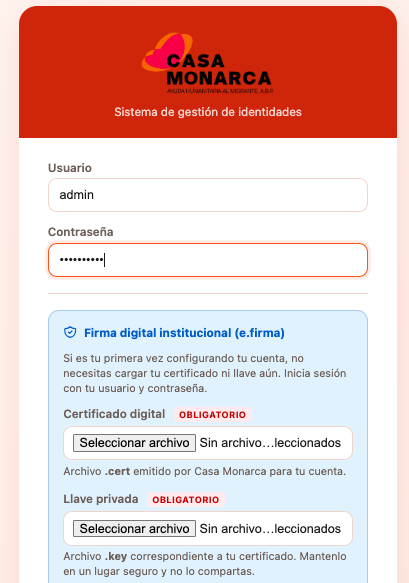
\includegraphics[width=0.55\textwidth]{login_form.png}
  \caption{Pantalla de login con los campos de usuario, contraseña y carga de \texttt{.cert}/\texttt{.key} (Nivel 1/2).}
  \label{fig:login_form}
\end{figure}

\paso{2}{Ingresar usuario y contraseña.}
Escribir el nombre de usuario y la contraseña asignados.

\paso{3}{Adjuntar \texttt{.cert} y \texttt{.key} (solo Nivel 1 y 2).}
Seleccionar ambos archivos en sus campos correspondientes. Son obligatorios para Administradores y Coordinadores.

% CAPTURA: login con .cert y .key seleccionados (Nivel 1/2).
\begin{figure}[H]\centering
  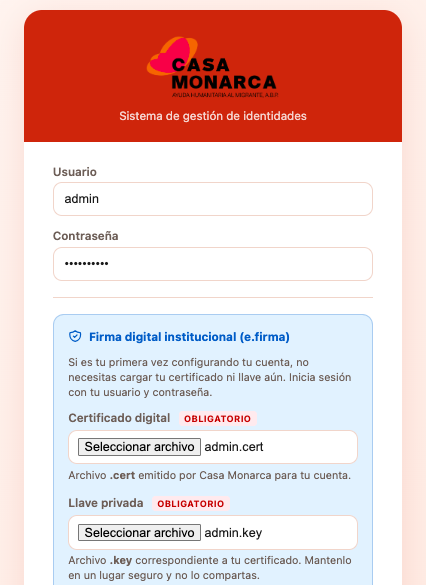
\includegraphics[width=0.55\textwidth]{login_cert_key.png}
  \caption{Formulario de login con los archivos \texttt{.cert} y \texttt{.key} seleccionados (Nivel 1/2).}
  \label{fig:login_cert_key}
\end{figure}

\paso{4}{Presionar ``Iniciar sesión'' y verificar la redirección.}
Si los datos son correctos, el sistema redirige según el nivel (Tabla~\ref{tab:redireccion}). Si son incorrectos, aparece un mensaje de error.

% CAPTURA: mensaje de error de login (contraseña incorrecta / cuenta revocada / archivos inválidos).
\begin{figure}[H]\centering
  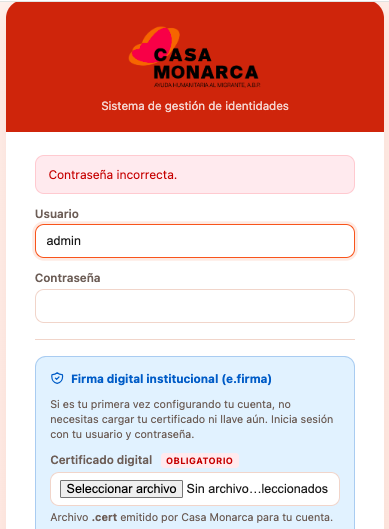
\includegraphics[width=0.55\textwidth]{login_error.png}
  \caption{Mensaje de error al iniciar sesión.}
  \label{fig:login_error}
\end{figure}

\section{Proceso de onboarding}
\label{sec:onboarding_comun}

El onboarding es el proceso obligatorio que todo colaborador nuevo debe completar antes de usar el sistema.

\begin{table}[H]\centering
\caption{Estados del proceso de onboarding.}
\label{tab:onboarding_estados}
\begin{tabularx}{\textwidth}{l l X}
\toprule
\textbf{Estado} & \textbf{Aplica a} & \textbf{Descripción}\\
\midrule
Pendiente           & Todos      & Formulario vacío; el colaborador debe llenarlo y enviarlo.\\
Enviado             & Todos      & En espera de revisión; no se puede editar.\\
Aprobado (descarga) & Nivel 1–2  & Descargar \texttt{.cert} y \texttt{.key}.\\
Relogin requerido   & Nivel 1–2  & Cerrar sesión y reingresar con las credenciales descargadas.\\
Aprobado            & Nivel 3–4  & Acceso directo al sistema con el nivel asignado.\\
Rechazado           & Todos      & Contactar al administrador.\\
\bottomrule
\end{tabularx}
\end{table}

\paso{1}{Llenar el formulario de onboarding (estado: Pendiente).}
Al iniciar sesión por primera vez el sistema redirige automáticamente al formulario. Registrar nombre, apellidos, teléfono (formato \texttt{+país-área-número}, ej. \texttt{+52-55-12345678}), cargar la identificación oficial en \textbf{PDF} y establecer la contraseña y la pregunta de seguridad.

\begin{nota}
La nueva contraseña debe cumplir: mínimo 8 caracteres, una mayúscula, un número y un carácter especial. La identificación oficial solo se acepta en formato PDF.
\end{nota}

% CAPTURA: formulario de onboarding vacío (nombre, apellidos, teléfono, INE PDF, contraseña, pregunta de seguridad).
\begin{figure}[H]\centering
  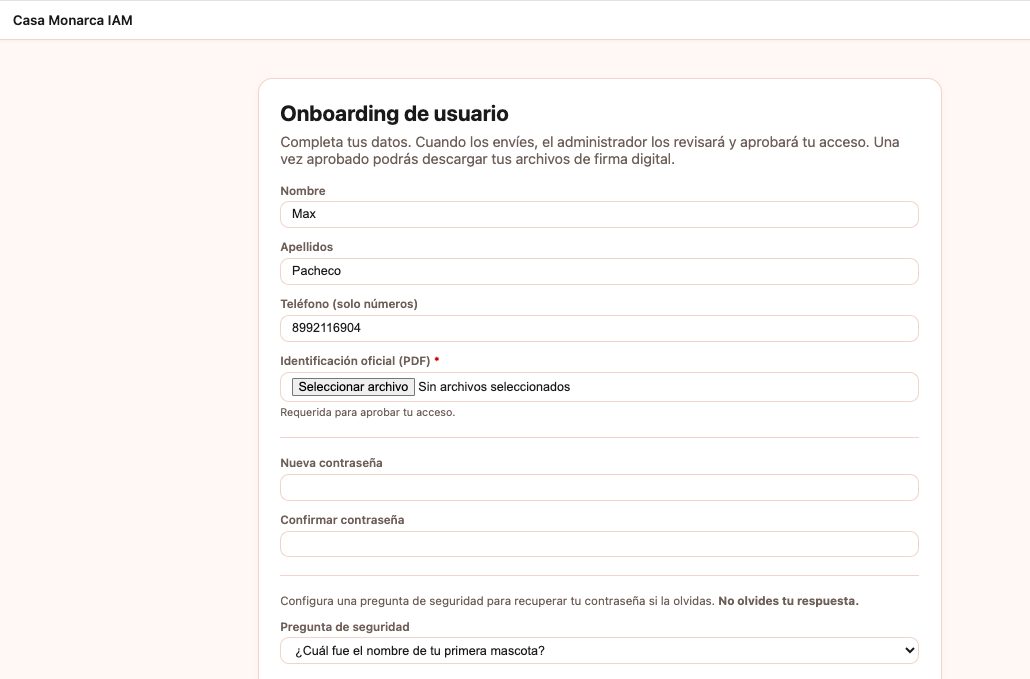
\includegraphics[width=0.55\textwidth]{onboarding_form.png}
  \caption{Formulario de onboarding con los campos de datos personales, contraseña y pregunta de seguridad.}
  \label{fig:onboarding_form}
\end{figure}

\paso{2}{Enviar el formulario (estado: Enviado).}
Hacer clic en ``Enviar onboarding''. El estado cambia a \textit{Enviado} y ya no se puede editar.

% CAPTURA: pantalla de confirmación de envío ("Tu solicitud está en revisión").
\begin{figure}[H]\centering
  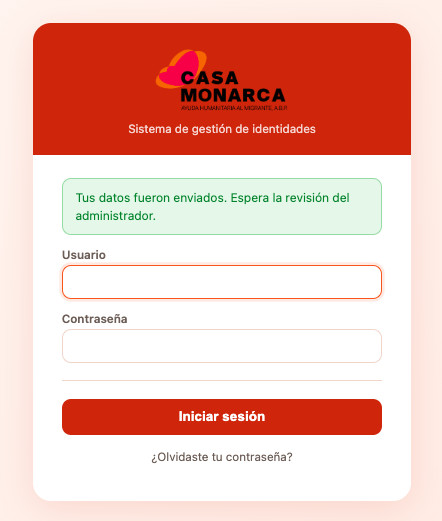
\includegraphics[width=0.65\textwidth]{onboarding_enviado.png}
  \caption{Pantalla de confirmación del estado ``Enviado'' con mensaje de espera.}
  \label{fig:onboarding_enviado}
\end{figure}

\paso{3}{Esperar aprobación.}
Un administrador o coordinador revisa los datos. Para aprobar, firma digitalmente con su contraseña y sus archivos \texttt{.cert} y \texttt{.key}.

\paso{4a}{Descargar credenciales (Nivel 1 y 2).}
Una vez aprobado y emitido el certificado, el sistema muestra la pantalla de descarga. Descargar \textbf{ambos} archivos (\texttt{.cert} y \texttt{.key}) y guardarlos en un lugar seguro.

% CAPTURA: pantalla de descarga con botones de .cert y .key.
\begin{figure}[H]\centering
  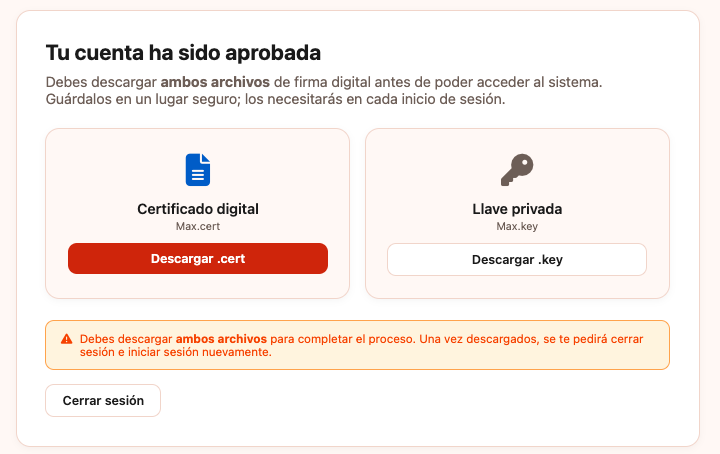
\includegraphics[width=0.75\textwidth]{onboarding_descarga.png}
  \caption{Pantalla de descarga de credenciales con los botones \texttt{.cert} y \texttt{.key} (Nivel 1/2).}
  \label{fig:onboarding_descarga}
\end{figure}

\paso{4b}{Cerrar sesión y reingresar (Relogin — Nivel 1 y 2).}
Tras descargar ambos archivos, cerrar sesión y volver a iniciar adjuntando los archivos descargados.

\paso{4c}{Acceso directo (Nivel 3 y 4).}
Los operativos y voluntarios acceden al sistema de inmediato tras la aprobación, sin descargar archivos.

\section{Recuperación de contraseña}

Disponible desde la pantalla de login. Requiere tener la pregunta de seguridad configurada previamente.

\paso{1}{Hacer clic en ``¿Olvidaste tu contraseña?'' en el login.}
\paso{2}{Ingresar el nombre de usuario exacto y hacer clic en ``Continuar''.}
\paso{3}{Responder la pregunta de seguridad correctamente.}
\paso{4}{Establecer la nueva contraseña} (debe cumplir las reglas de contraseña fuerte) y hacer clic en ``Restablecer''.

% CAPTURA: pantalla de recuperación — campo de usuario (paso 2).
\begin{figure}[H]\centering
  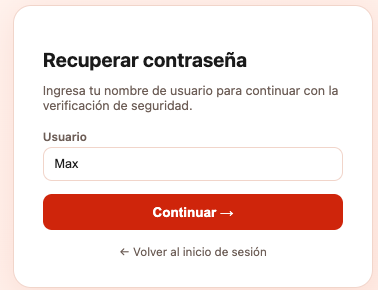
\includegraphics[width=0.55\textwidth]{recovery_usuario.png}
  \caption{Formulario de recuperación de contraseña — campo de nombre de usuario.}
  \label{fig:recovery_usuario}
\end{figure}

% CAPTURA: pantalla de recuperación — pregunta de seguridad y campo de respuesta (paso 3).
\begin{figure}[H]\centering
  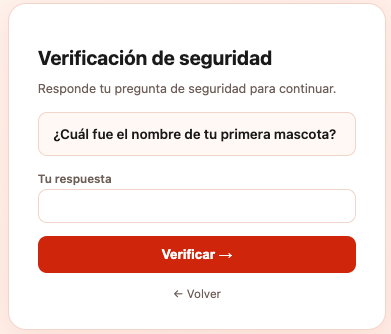
\includegraphics[width=0.55\textwidth]{recovery_pregunta.png}
  \caption{Pregunta de seguridad y campo de respuesta en el flujo de recuperación.}
  \label{fig:recovery_pregunta}
\end{figure}


\section{Cambio de contraseña}

Disponible para cualquier usuario con sesión activa. Ir al menú de perfil (ícono superior derecho) → \textbf{Cambiar contraseña}. Ingresar la contraseña actual, la nueva y su confirmación.

\section{Configuración de pregunta de seguridad}

Disponible en el menú de perfil → \textbf{Cambiar pregunta de seguridad}. Seleccionar una de las 8 preguntas disponibles, ingresar la respuesta y confirmarla. Se puede actualizar en cualquier momento.

% CAPTURA: formulario de pregunta de seguridad (selector de pregunta, campo de respuesta y confirmación).
\begin{figure}[H]\centering
  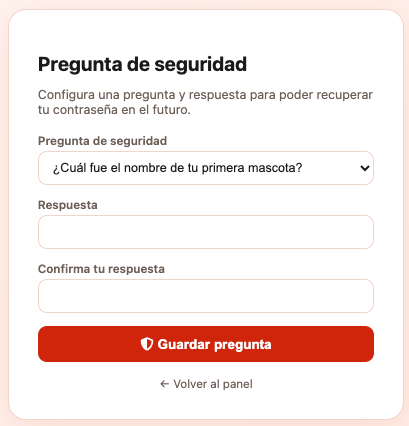
\includegraphics[width=0.55\textwidth]{pregunta_seguridad.png}
  \caption{Formulario de configuración de pregunta de seguridad.}
  \label{fig:pregunta_seguridad}
\end{figure}

% ============================================================================
%  PARTE II ─ MANUAL DEL ADMINISTRADOR (Nivel 1)
% ============================================================================
\part{Manual del Administrador --- Nivel 1}

\chapter{Gestión de colaboradores}
% ──────────────────────────────────────────────────────────────────
\paraadmin

El Administrador tiene acceso total a todos los colaboradores del sistema, sin restricción de área.

\section{Dashboard de colaboradores}

El dashboard muestra las tarjetas de estadísticas (total, activos, revocados, eliminados), una barra de búsqueda por texto libre (nombre, apellido, usuario o correo) y filtros por área, nivel de acceso y estado. Desde aquí se accede al alta de colaboradores, a la auditoría y a los onboardings pendientes.

% CAPTURA: dashboard de colaboradores con tarjetas de estadísticas, buscador y listado.
\begin{figure}[H]\centering
  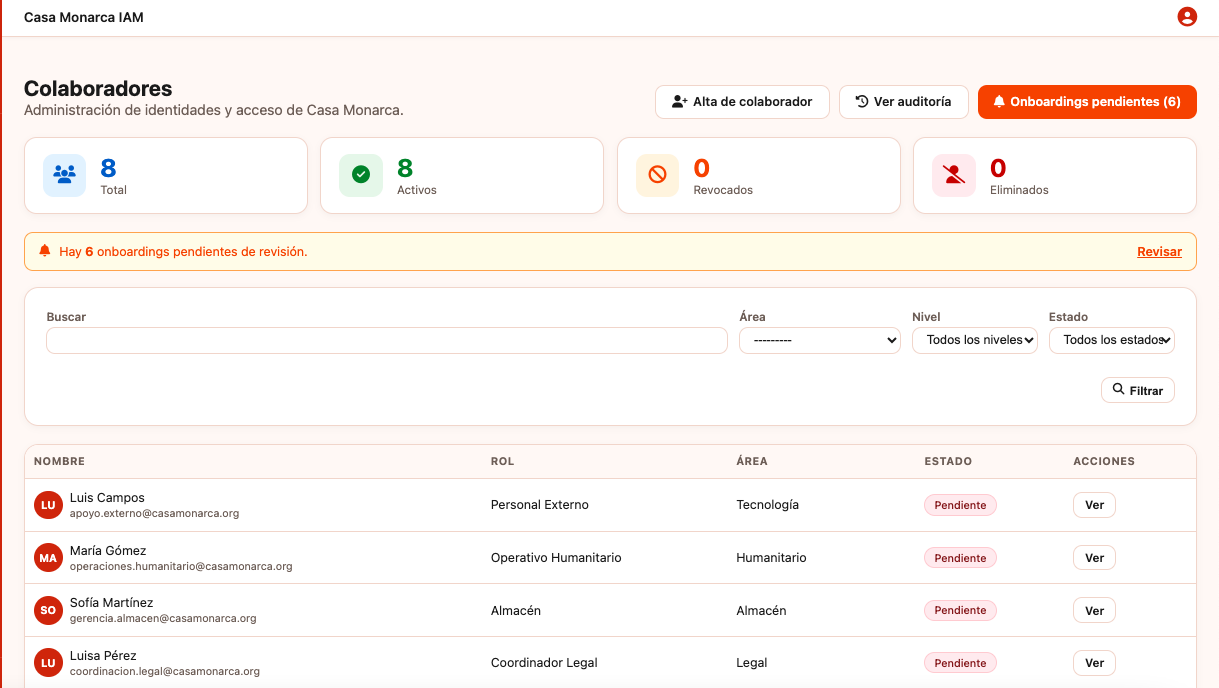
\includegraphics[width=0.95\textwidth]{dashboard_admin.png}
  \caption{Dashboard del Administrador con estadísticas, filtros y listado completo de colaboradores.}
  \label{fig:dashboard_admin}
\end{figure}

\section{Alta de colaboradores}

\paso{1}{Clic en ``+ Alta de colaborador'' desde el dashboard.}

\paso{2}{Completar el formulario de alta.}
Campos: nombre de usuario, nombre, apellido, correo institucional, teléfono (solo dígitos), área, nivel de acceso, rol, puesto y fecha de ingreso. Para Nivel 1, seleccionar también el tipo de cuenta admin (Producción o Contingencias).

% CAPTURA: formulario de alta de colaborador con todos los campos.
\begin{figure}[H]\centering
  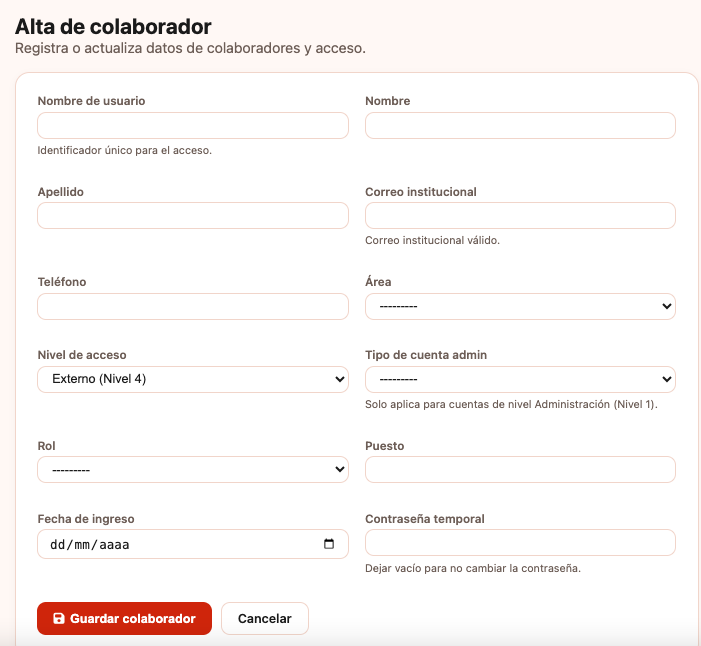
\includegraphics[width=0.9\textwidth]{alta_form.png}
  \caption{Formulario de alta de colaborador con los campos obligatorios.}
  \label{fig:alta_form}
\end{figure}

\paso{3}{Guardar.}
El sistema crea la cuenta con estado de onboarding \textit{Pendiente}, genera una \textbf{contraseña temporal aleatoria} y la muestra \textbf{una sola vez} en la pantalla de confirmación. Copiarla y entregarla de forma segura al colaborador.

% CAPTURA: pantalla de confirmación con la contraseña temporal (se muestra una sola vez).
\begin{figure}[H]\centering
  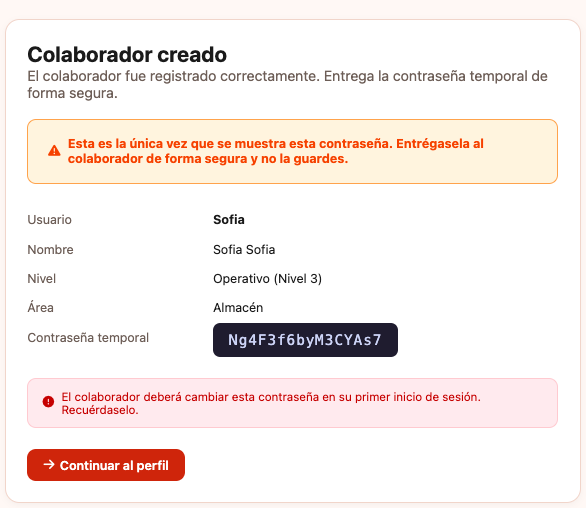
\includegraphics[width=0.8\textwidth]{alta_password_temporal.png}
  \caption{Pantalla de confirmación tras el alta con la contraseña temporal (solo visible una vez).}
  \label{fig:alta_password_temporal}
\end{figure}

\section{Vista de detalle y gestión de un colaborador}

Hacer clic sobre un colaborador del listado para abrir su vista de detalle. Desde ahí se pueden ejecutar todas las acciones administrativas.

% CAPTURA: vista de detalle completa de un colaborador (datos personales, estado, onboarding, certificado, auditoría).
\begin{figure}[H]\centering
  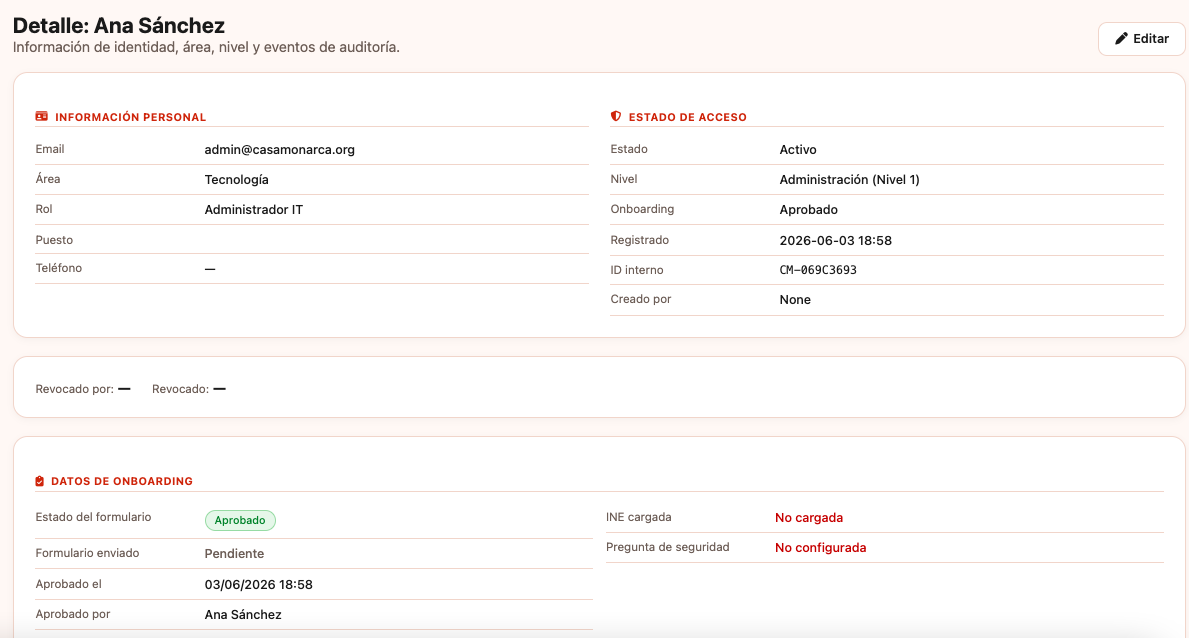
\includegraphics[width=0.95\textwidth]{detalle_colaborador.png}
  \caption{Vista de detalle de un colaborador con datos, estado de onboarding, certificado e historial.}
  \label{fig:detalle_colaborador}
\end{figure}

\begin{table}[H]\centering
\caption{Acciones disponibles en la vista de detalle del colaborador (Nivel 1).}
\label{tab:acciones_admin}
\begin{tabularx}{\textwidth}{l X}
\toprule
\textbf{Acción} & \textbf{Descripción}\\
\midrule
Editar               & Actualiza datos del colaborador.\\
Activar / Desactivar & Cambia el estado activo de la cuenta (reversible).\\
Revocar              & Bloquea el acceso; el registro permanece. Reversible.\\
Eliminar             & Baja lógica permanente. No reversible desde la interfaz.\\
Emitir certificado   & Genera el certificado digital (gestión avanzada en Cap.~\ref{ch:certmgmt}).\\
Validar certificado  & Verifica si el certificado vigente es válido.\\
\bottomrule
\end{tabularx}
\end{table}

\section{Onboardings pendientes}

Clic en \textbf{Onboardings pendientes} desde el dashboard o el menú. Se listan los colaboradores que aún no completaron o no fueron aprobados. Para aprobar un onboarding completo, hacer clic en \textbf{Revisar y aprobar}, ingresar la contraseña y adjuntar \texttt{.cert} y \texttt{.key}.

% CAPTURA: pantalla de revisión de onboarding completo con campos de contraseña y .cert/.key.
\begin{figure}[H]\centering
  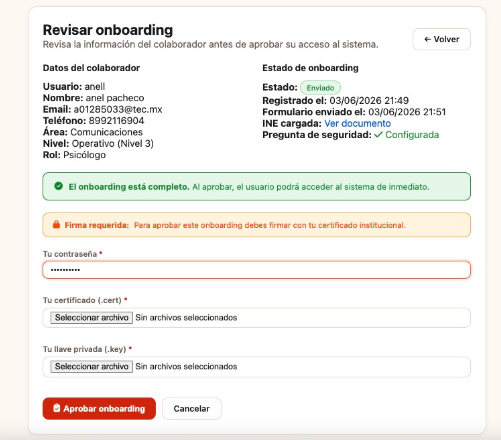
\includegraphics[width=0.85\textwidth]{aprobar_onboarding.png}
  \caption{Pantalla para aprobación firmada de onboarding con contraseña y credenciales del aprobador.}
  \label{fig:aprobar_onboarding}
\end{figure}

\section{Auditoría IAM}

Accesible desde el menú → \textbf{Auditoría}. Muestra todos los eventos del sistema IAM (hasta 500 registros) con filtros por rango de fechas, acción, actor y usuario objetivo.

% CAPTURA: pantalla de auditoría con la tabla de eventos y los filtros aplicados.
\begin{figure}[H]\centering
  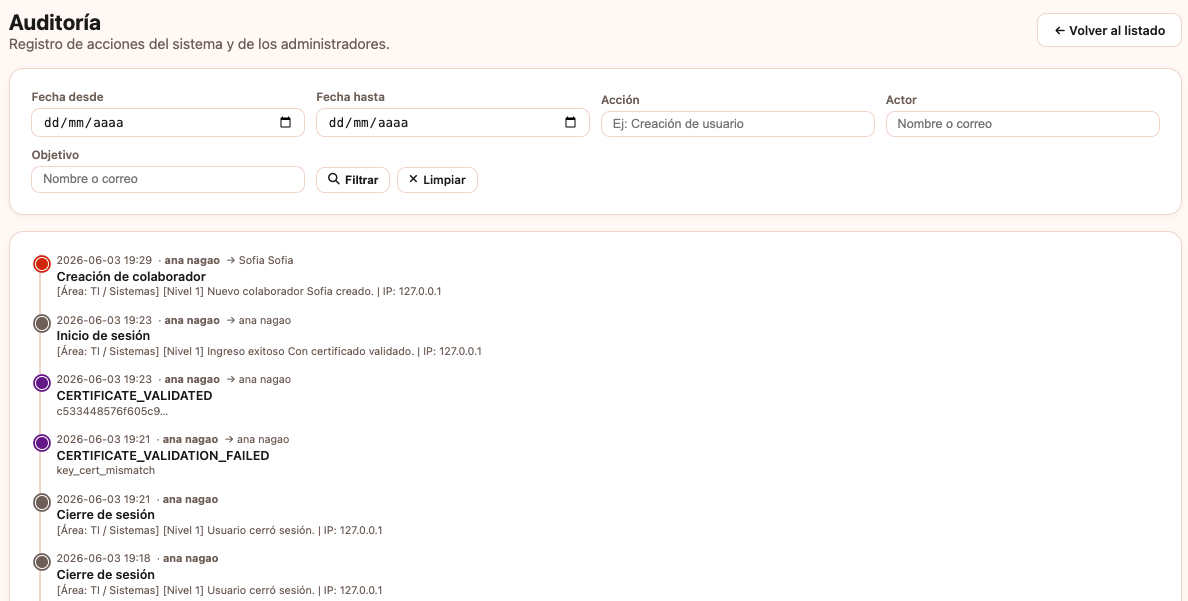
\includegraphics[width=0.95\textwidth]{auditoria_iam.png}
  \caption{Módulo de auditoría IAM con filtros y tabla de eventos.}
  \label{fig:auditoria_iam}
\end{figure}

% ──────────────────────────────────────────────────────────────────
\chapter{Gestión de certificados digitales}
\label{ch:certmgmt}
% ──────────────────────────────────────────────────────────────────
\paraadmin

Los certificados digitales se emiten automáticamente durante el proceso de onboarding de los colaboradores de Nivel 1 y 2. Este módulo permite al Administrador \textbf{monitorear y controlar} los certificados ya emitidos: consultarlos, suspenderlos temporalmente, reactivarlos, revocarlos o darlos de baja. Es accesible desde el menú → \textbf{Certificados}.

\section{Listado de certificados}

El listado muestra todos los certificados del sistema con tarjetas de resumen (Activos, Suspendidos, Revocados, Expirados e Inactivos) y una tabla con el usuario vinculado, área, número de serie, estado, fecha de emisión y fecha de vencimiento. Permite filtrar por estado, área, rango de fechas y buscar por nombre, apellido, usuario o número de serie.

% CAPTURA: pantalla de Gestión de certificados con las tarjetas de resumen y la tabla
%          (columnas: Usuario, Área, Nº Serie, Estado, Emitido, Vence, Acciones).
\begin{figure}[H]\centering
  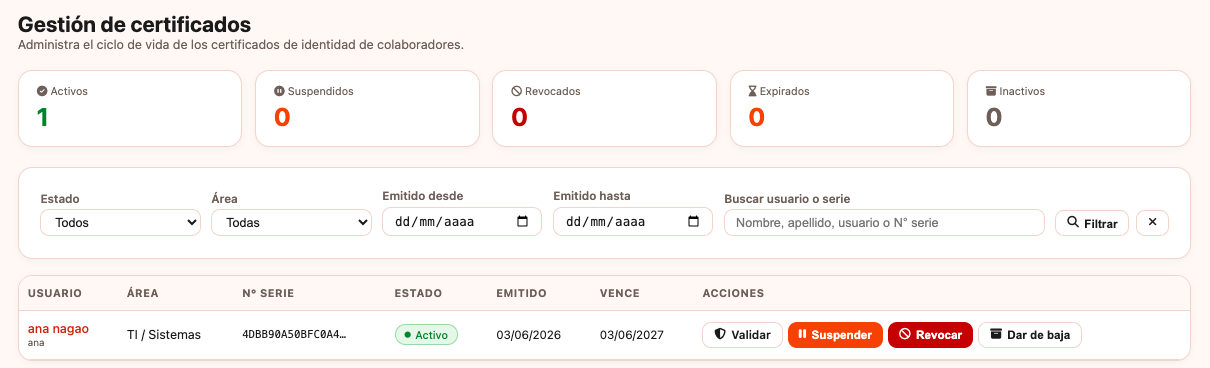
\includegraphics[width=0.95\textwidth]{cert_lista.png}
  \caption{Listado de certificados digitales con tarjetas de resumen, filtros y acciones.}
  \label{fig:cert_lista}
\end{figure}

\section{Acciones sobre un certificado}

Desde el listado, cada certificado tiene las siguientes acciones disponibles según su estado actual:

\begin{table}[H]\centering
\caption{Acciones disponibles sobre un certificado y estado resultante.}
\label{tab:cert_ciclo}
\begin{tabularx}{\textwidth}{l l X}
\toprule
\textbf{Acción} & \textbf{Estado resultante} & \textbf{Descripción}\\
\midrule
Validar     & (sin cambio) & Verifica que el certificado sea criptográficamente válido.\\
Suspender   & Suspendido   & Bloqueo temporal; el usuario no puede iniciar sesión. Reversible.\\
Reactivar   & Activo       & Levanta la suspensión; el usuario recupera el acceso.\\
Revocar     & Revocado     & Revocación permanente por razones de seguridad. No reversible.\\
Dar de baja & Inactivo     & Baja administrativa (colaborador fuera o cert reemplazado). No reversible.\\
\bottomrule
\end{tabularx}
\end{table}

\begin{nota}
Las acciones \textbf{Revocar} y \textbf{Dar de baja} son permanentes e irreversibles. Usar \textbf{Suspender} cuando se necesite bloquear el acceso de forma temporal sin invalidar definitivamente el certificado.
\end{nota}

\subsection*{Validar un certificado}
Hacer clic en \textbf{Validar}. El sistema comprueba la firma criptográfica y muestra el resultado de la verificación.

% CAPTURA: resultado de la validación (mensaje de éxito o de error de verificación).
\begin{figure}[H]\centering
  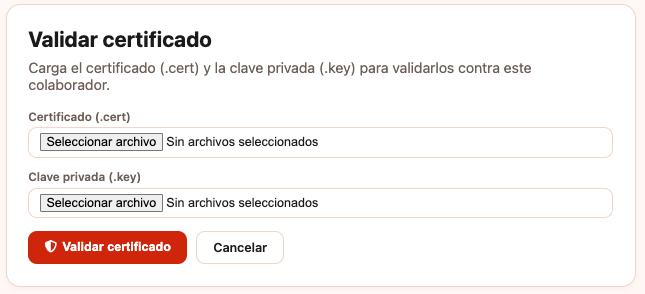
\includegraphics[width=0.85\textwidth]{cert_validar.png}
  \caption{Resultado del botón de validación.}
  \label{fig:cert_validar}
\end{figure}

\subsection*{Suspender un certificado}
Hacer clic en \textbf{Suspender} y confirmar. El usuario vinculado no podrá iniciar sesión hasta que el certificado sea reactivado.

% CAPTURA: listado con el certificado en estado "Suspendido" tras confirmar la acción.
\begin{figure}[H]\centering
  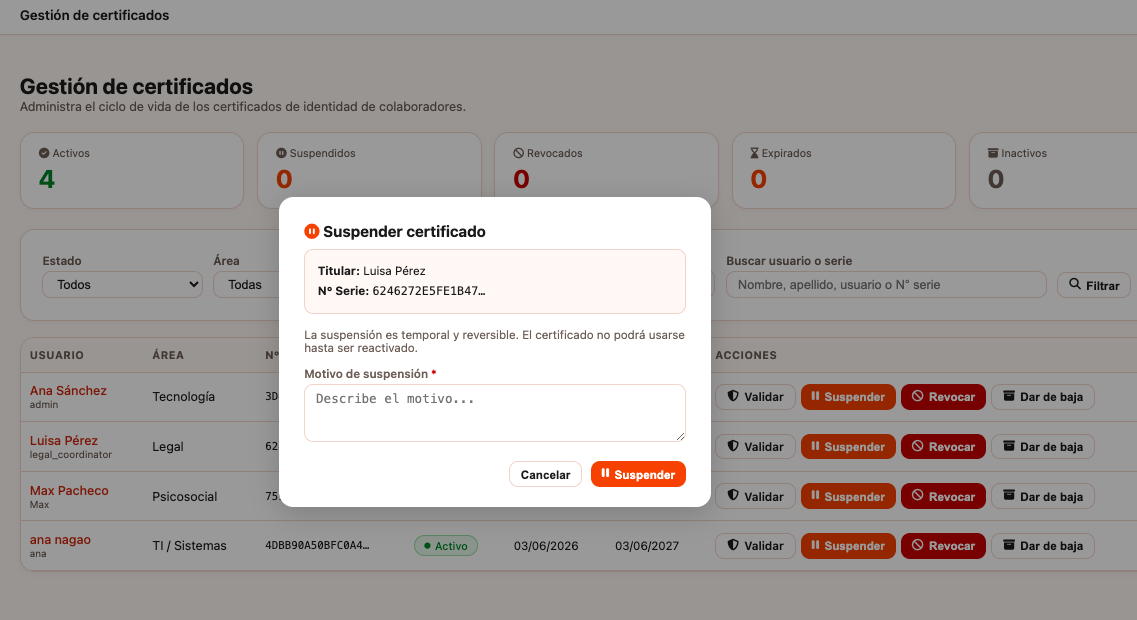
\includegraphics[width=0.85\textwidth]{cert_suspender.png}
  \caption{Certificado a suspender.}
  \label{fig:cert_suspender}
\end{figure}

\subsection*{Reactivar un certificado suspendido}
Hacer clic en \textbf{Reactivar} y confirmar. El certificado vuelve a estado \textit{Activo} y el usuario puede iniciar sesión nuevamente.

% CAPTURA: listado con el certificado en estado "Activo" tras reactivar.
\begin{figure}[H]\centering
  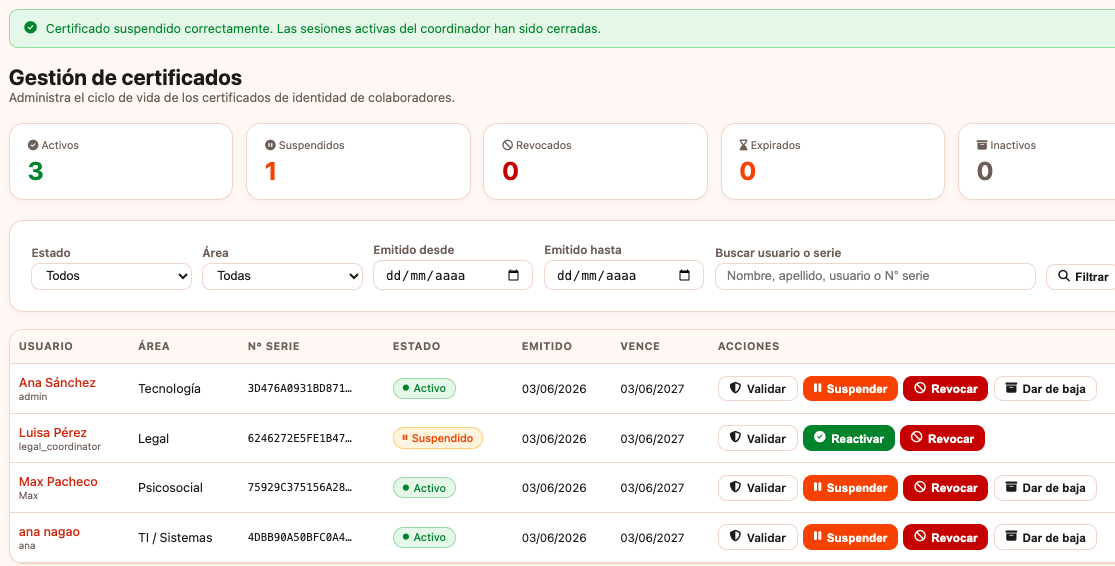
\includegraphics[width=0.85\textwidth]{cert_reactivar.png}
  \caption{Certificado a reactivar con botón de  ``Reactivar''.}
  \label{fig:cert_reactivar}
\end{figure}

\subsection*{Revocar un certificado}
Hacer clic en \textbf{Revocar} y confirmar. La revocación es permanente: el certificado queda invalidado definitivamente. Si el colaborador necesita volver a acceder al sistema deberá completar un nuevo proceso de onboarding.

\subsection*{Dar de baja un certificado}
Hacer clic en \textbf{Dar de baja} y confirmar. Usar cuando el colaborador sale de la organización o cuando el certificado es reemplazado por uno nuevo. No reversible.

\section{Auditoría de un certificado}

Hacer clic en el número de serie o en el nombre del usuario para acceder al historial completo de eventos sobre ese certificado: emisión, validaciones, suspensiones, reactivaciones, revocación o baja, con fecha y responsable de cada acción.

% CAPTURA: pantalla de auditoría de un certificado (tabla con fecha, acción y actor).
\begin{figure}[H]\centering
  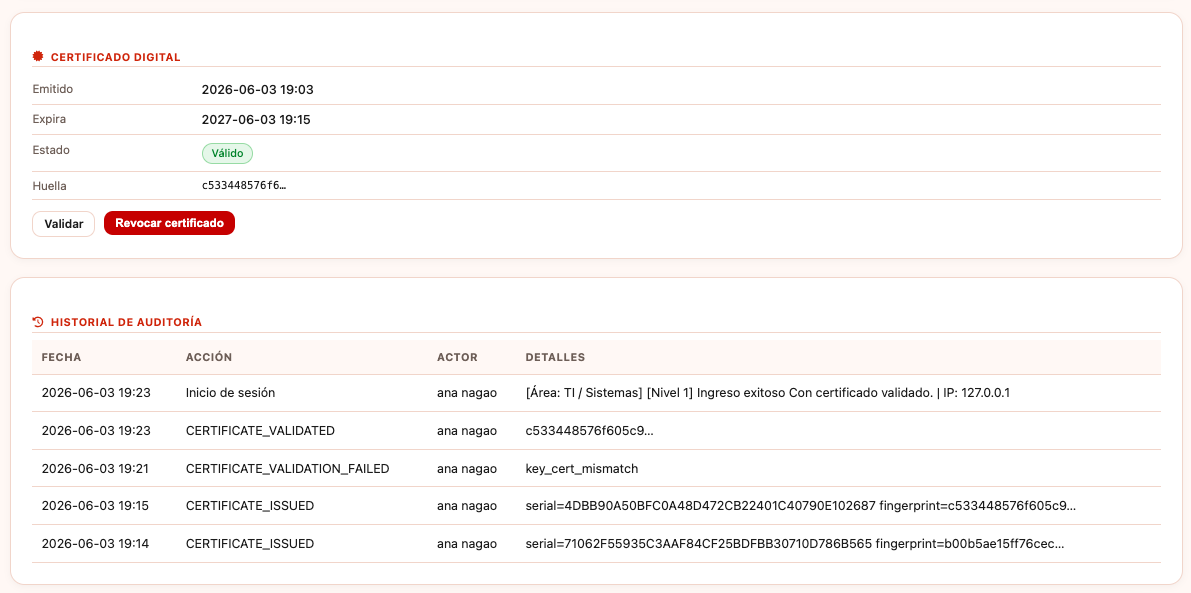
\includegraphics[width=0.95\textwidth]{cert_auditoria.png}
  \caption{Historial de auditoría de un certificado digital con todas las acciones registradas.}
  \label{fig:cert_auditoria}
\end{figure}
% ──────────────────────────────────────────────────────────────────
\chapter{Registro de migrantes --- vista del Administrador}
\label{ch:migrante_admin}
% ──────────────────────────────────────────────────────────────────
\paraadmin

\section{Campos del formulario de registro}
\label{sec:campos_migrante}

El formulario de registro contiene los siguientes campos. Los marcados con \textbf{(cifrado)} se almacenan encriptados en la base de datos.

\begin{table}[H]\centering
\caption{Campos del formulario de registro de migrante.}
\label{tab:campos_migrante}
\begin{tabularx}{\textwidth}{l X l}
\toprule
\textbf{Campo} & \textbf{Descripción} & \textbf{Notas}\\
\midrule
Nombre                & Nombre(s) del beneficiario & Cifrado, máx. 50 car.\\
Primer apellido       & Primer apellido & Cifrado, máx. 50 car.\\
Segundo apellido      & Segundo apellido & Cifrado; si no aplica se registra ``X''\\
Fecha de nacimiento   & Fecha de nacimiento & Cifrada\\
Género                & Femenino / Masculino / No binario / LGBTIQ\texttt{+} & \\
País de origen        & País de origen & Cifrado\\
Departamento/Estado   & Estado o departamento de origen & \\
Teléfono              & Formato \texttt{+país-área-número} & Cifrado; ej. \texttt{+52-55-12345678}\\
Fecha de servicio     & Fecha en que se atendió al beneficiario & \\
Estado civil          & Soltero/a, Casado/a, Unión libre, Divorciado/a, Viudo/a & \\
Grupo de edad         & Infancia / Adolescencia / Adulto / Adulto mayor & \\
Grupo poblacional     & Adulto, Adulto mayor, Niña/Niño acompañado, Adolescente, NNA no acompañado & \\
Consentimiento        & Aviso de Privacidad aceptado & Obligatorio\\
Método de consentimiento & Digital / Verbal con testigo / Firmado en papel & \\
Captura por intermediario & Marcar si el beneficiario no puede operar el sistema & \\
\bottomrule
\end{tabularx}
\end{table}

\begin{nota}
Los campos cifrados (nombre, apellidos, fecha de nacimiento, teléfono y país de origen) se almacenan encriptados en la base de datos. El listado de registros solo puede buscarse por \textbf{identificador interno} (\texttt{CM-XXXXXXXX}), no por nombre, porque este está cifrado.
\end{nota}

\section{Crear un nuevo registro (Nivel 1 y 2 — directo)}

\paso{1}{Menú → \textbf{Nuevo Registro}.}
Se abre el formulario completo.

% CAPTURA: formulario de nuevo registro con todos los campos (nombre, apellidos, fecha nacimiento, género, país, etc.)
\begin{figure}[H]\centering
  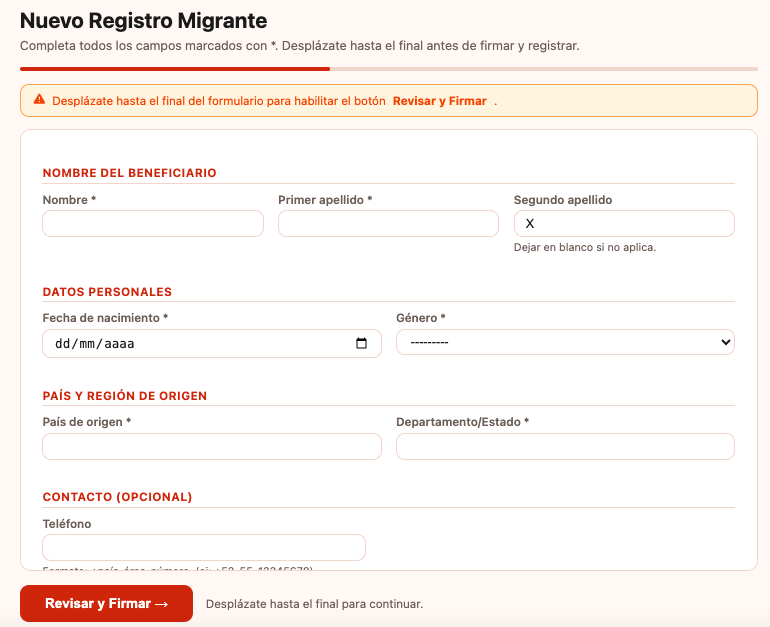
\includegraphics[width=0.9\textwidth]{migrante_form.png}
  \caption{Formulario de nuevo registro de migrante con los campos vacíos.}
  \label{fig:migrante_form}
\end{figure}

\paso{2}{Completar todos los campos y aceptar el Aviso de Privacidad.}
Llenar los datos, seleccionar el método de captura del consentimiento y, si el beneficiario no puede operar el sistema, marcar la casilla de captura por intermediario.

% CAPTURA: sección de consentimiento al pie del formulario (casilla de Aviso, selector de método, casilla de intermediario).
\begin{figure}[H]\centering
  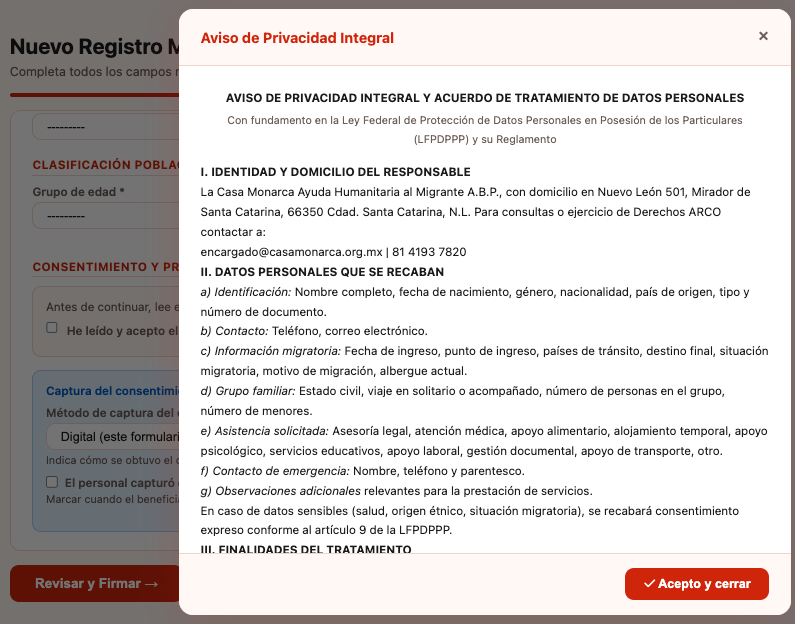
\includegraphics[width=0.75\textwidth]{migrante_consent.png}
  \caption{Sección de consentimiento de datos personales al pie del formulario.}
  \label{fig:migrante_consent}
\end{figure}

\paso{3}{Pantalla de revisión y confirmación.}
El sistema muestra todos los datos agrupados para revisión. Ingresar la contraseña y hacer clic en \textbf{Confirmar y firmar registro}. El sistema calcula el hash del expediente y lo firma con ECDSA.

% CAPTURA: pantalla de revisión con los datos agrupados y el campo de contraseña al pie.
\begin{figure}[H]\centering
  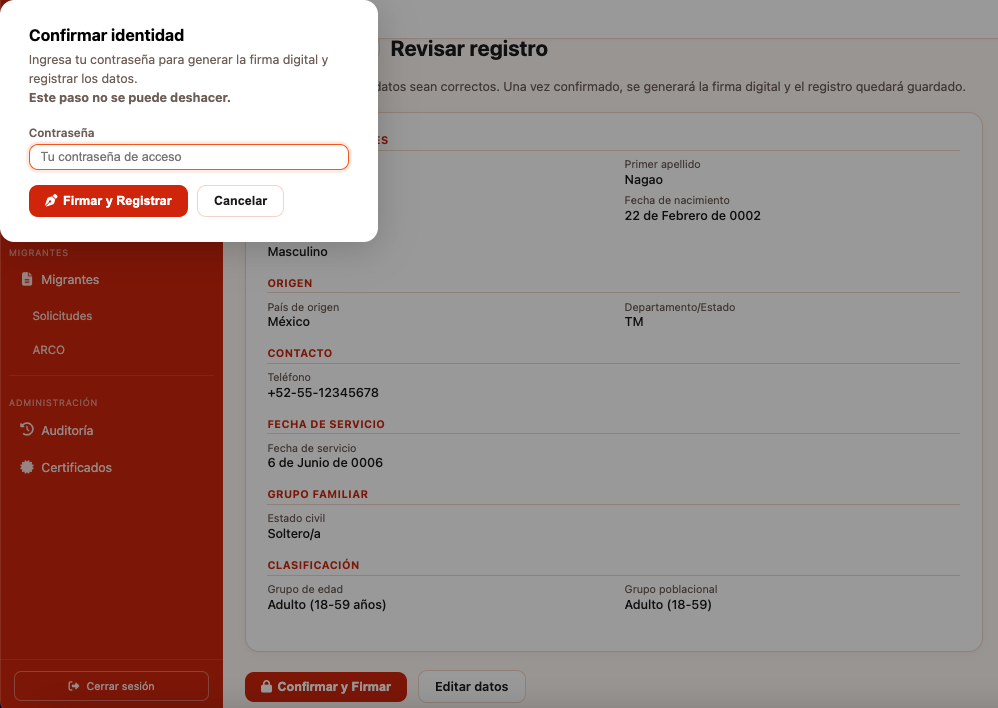
\includegraphics[width=0.9\textwidth]{migrante_review.png}
  \caption{Pantalla de revisión y confirmación con contraseña antes de firmar el registro.}
  \label{fig:migrante_review}
\end{figure}

\paso{4}{Pantalla de éxito.}
El sistema muestra el identificador interno generado (\texttt{CM-XXXXXXXX}) y un enlace al ticket de seguimiento.

% CAPTURA: pantalla de éxito con el identificador interno y el enlace al ticket.
\begin{figure}[H]\centering
  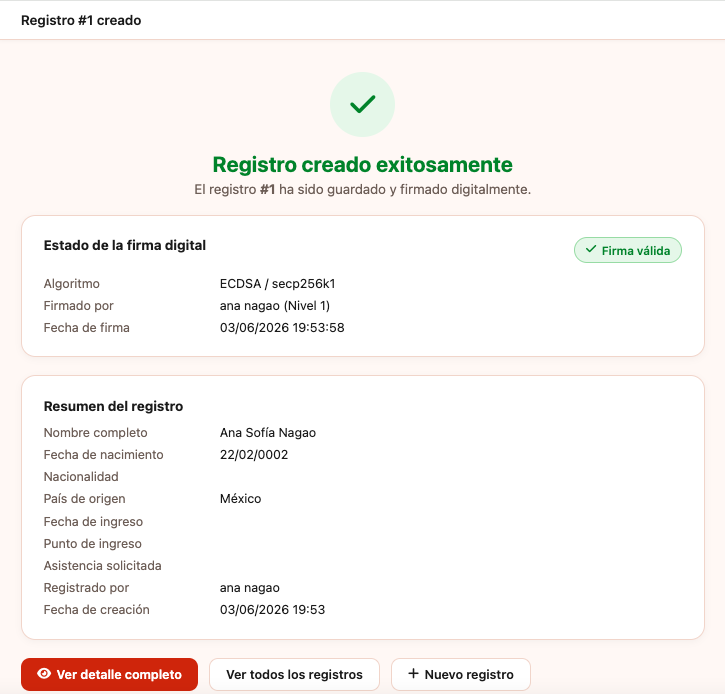
\includegraphics[width=0.75\textwidth]{migrante_exito.png}
  \caption{Pantalla de registro exitoso con el número de registro.}
  \label{fig:migrante_exito}
\end{figure}

\section{Listado y búsqueda}

Menú → \textbf{Migrantes}. Muestra todos los registros activos. La búsqueda es por \textbf{folio} del registro (ej: \texttt{MIG-XXXX}). En la parte superior derecha aparece el botón \textbf{+ Nuevo registro}.


% CAPTURA: listado de registros con columna de ID interno, género, grupo de edad, grupo poblacional, fecha de servicio y acciones.
\begin{figure}[H]\centering
  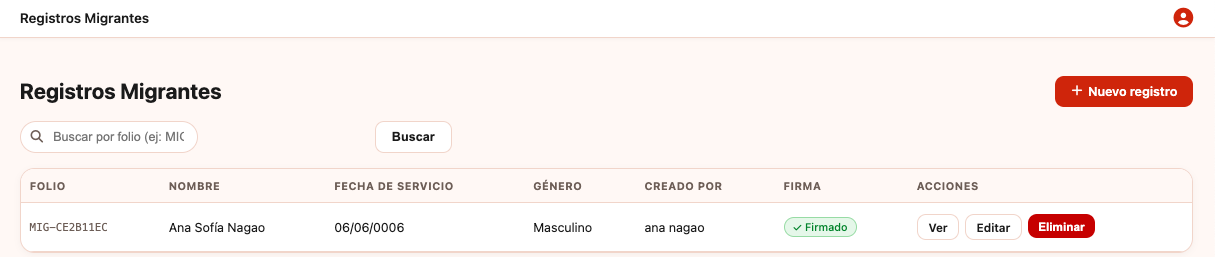
\includegraphics[width=0.95\textwidth]{migrante_lista.png}
  \caption{Listado de registros de migrantes con buscador por identificador interno.}
  \label{fig:migrante_lista}
\end{figure}

\section{Vista de detalle del registro}

Hacer clic en un registro del listado. El detalle muestra el expediente organizado en cinco secciones: \textbf{Datos personales} (fecha de nacimiento, género, estado civil), \textbf{Origen} (país de origen, departamento/estado), \textbf{Contacto} (teléfono), \textbf{Atención} (fecha de servicio, grupo de edad, grupo poblacional) y \textbf{Metadatos} (creado por, fecha de creación, última actualización y registro del consentimiento). Al pie se muestra el bloque de \textbf{Firma digital ECDSA} con el firmante y la fecha de firma.

Desde esta vista están disponibles las siguientes acciones: \textbf{Expediente / Historial}, \textbf{Editar}, \textbf{Nueva solicitud ARCO} y \textbf{Eliminar}.

% CAPTURA: vista de detalle de un registro con las secciones Datos personales, Origen,
%          Contacto, Atención, Metadatos, bloque de Firma ECDSA y los botones de acción.
\begin{figure}[H]\centering
  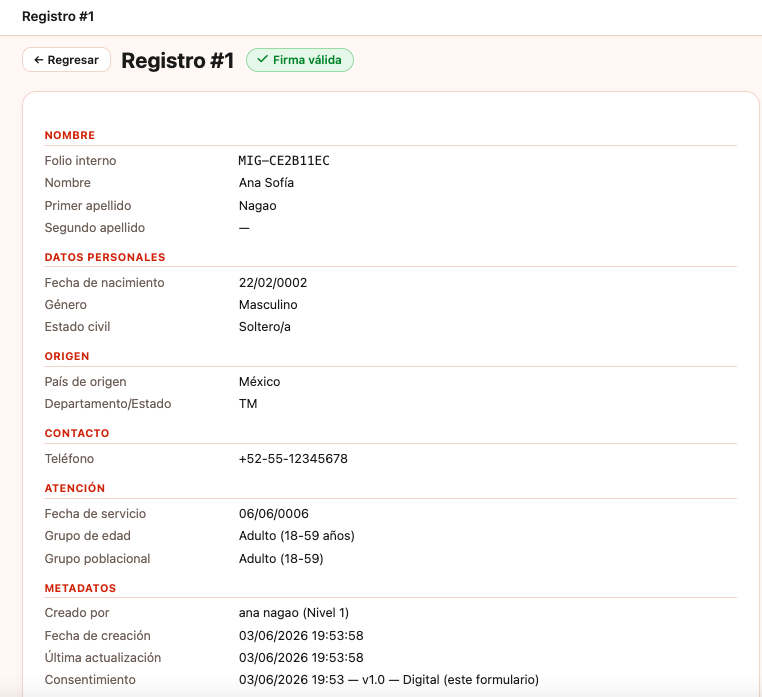
\includegraphics[width=0.95\textwidth]{migrante_detalle.png}
  \caption{Vista de detalle de un registro de migrante con datos, firma ECDSA y acciones disponibles.}
  \label{fig:migrante_detalle}
\end{figure}

\section{Editar un registro}

Desde el detalle, clic en \textbf{Editar}. El formulario carga con los datos actuales. Al guardar, el sistema \textbf{recalcula y actualiza la firma ECDSA} del registro automáticamente.

% CAPTURA: formulario de edición con datos precargados y botón "Guardar".
\begin{figure}[H]\centering
  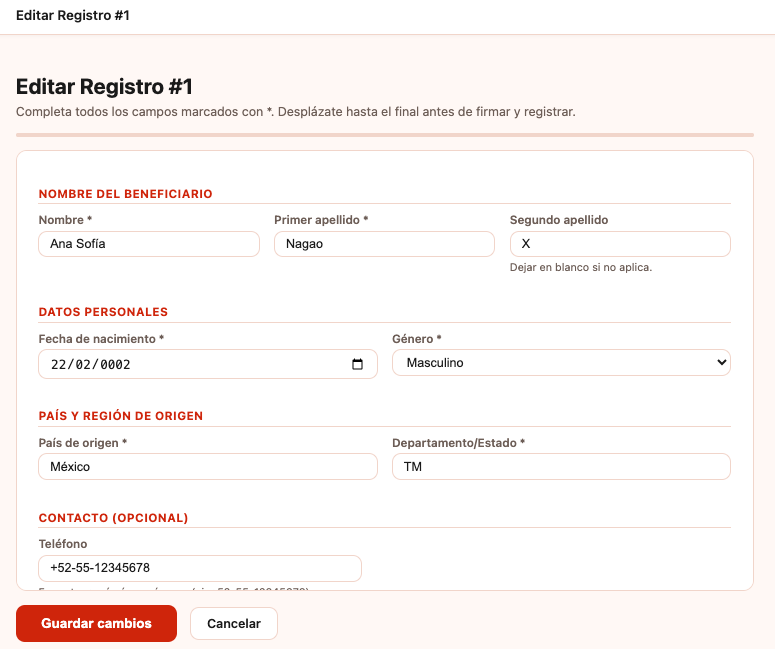
\includegraphics[width=0.9\textwidth]{migrante_editar.png}
  \caption{Formulario de edición de un registro con los datos actuales precargados.}
  \label{fig:migrante_editar}
\end{figure}

\section{Eliminar un registro}

Desde el detalle, clic en \textbf{Eliminar} y confirmar. La eliminación es \textbf{lógica}: el registro se marca como eliminado y deja de aparecer en el listado activo. El Administrador puede verlo en \textbf{Registros eliminados}.

\section{Expediente completo del migrante}
\label{sec:expediente}

Disponible para Nivel 1 y 2. Desde el detalle → \textbf{Expediente}. Muestra la línea de tiempo completa de todos los eventos del registro: creaciones, ediciones, consultas, solicitudes ARCO y workflows asociados.

% CAPTURA: pantalla de expediente con la línea de tiempo de eventos del registro.
\begin{figure}[H]\centering
  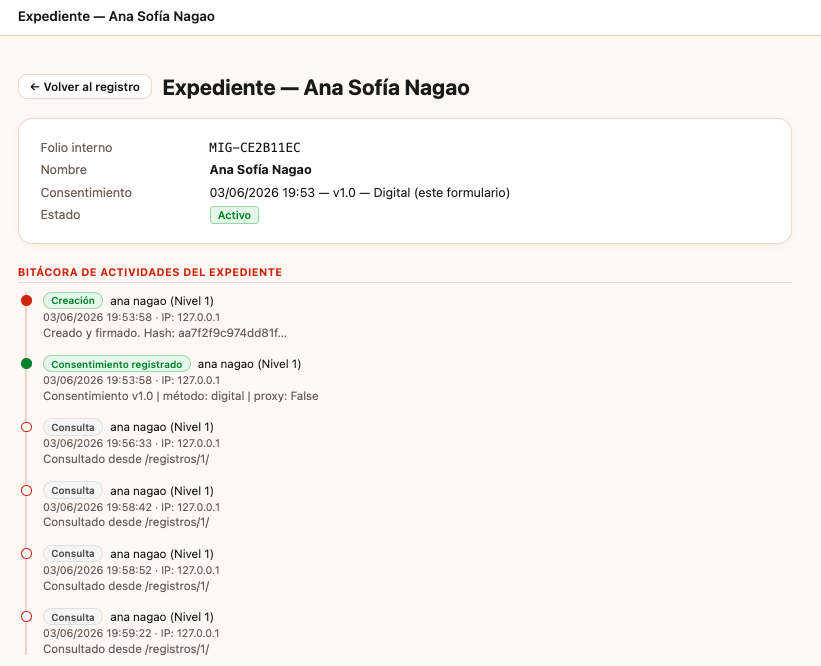
\includegraphics[width=0.95\textwidth]{expediente.png}
  \caption{Expediente completo del migrante con la línea de tiempo de eventos y documentos vinculados.}
  \label{fig:expediente}
\end{figure}

\chapter{Solicitudes de cambio --- Workflow (Administrador)}
% ──────────────────────────────────────────────────────────────────
\paraadmin

El Administrador ve y puede actuar sobre \textbf{todas} las solicitudes del sistema.

\begin{table}[H]\centering
\caption{Estados de una solicitud en el flujo de aprobación.}
\label{tab:workflow_estados}
\begin{tabularx}{\textwidth}{l X}
\toprule
\textbf{Estado} & \textbf{Descripción}\\
\midrule
Enviado              & Solicitud creada; esperando revisión.\\
En revisión          & Un aprobador está evaluándola.\\
Escalado             & Escalada al nivel superior.\\
Aprobado             & Todos los niveles requeridos aprobaron; pendiente de ejecución.\\
Firmado digitalmente & Aprobación firmada con \texttt{.cert} y \texttt{.key}.\\
Ejecutado            & Acción aplicada al registro.\\
Rechazado            & Al menos un nivel rechazó la solicitud.\\
\bottomrule
\end{tabularx}
\end{table}

\section{Listado de solicitudes}

Menú → \textbf{Solicitudes}. Se muestra la tabla completa con tipo de acción, registro afectado, solicitante, estado y fecha.

% CAPTURA: listado de solicitudes con columnas de número, tipo, registro, solicitante, estado y fecha.
\begin{figure}[H]\centering
  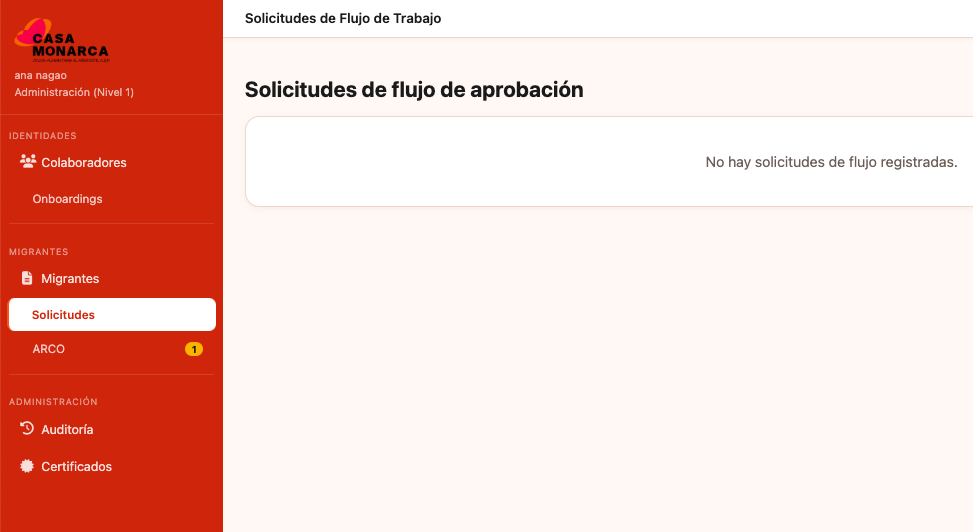
\includegraphics[width=0.95\textwidth]{workflow_lista.png}
  \caption{Listado de solicitudes de cambio con estado y acciones.}
  \label{fig:workflow_lista}
\end{figure}

\section{Aprobar o rechazar una solicitud}

\paso{1}{Desde el listado, clic en la solicitud → clic en \textbf{Decidir}.}

\paso{2}{Seleccionar Aprobar o Rechazar, agregar notas, ingresar la contraseña y adjuntar \texttt{.cert} y \texttt{.key} (para aprobaciones).}

% CAPTURA: pantalla de decisión con radio buttons, notas, contraseña y campos .cert/.key.
\begin{figure}[H]\centering
  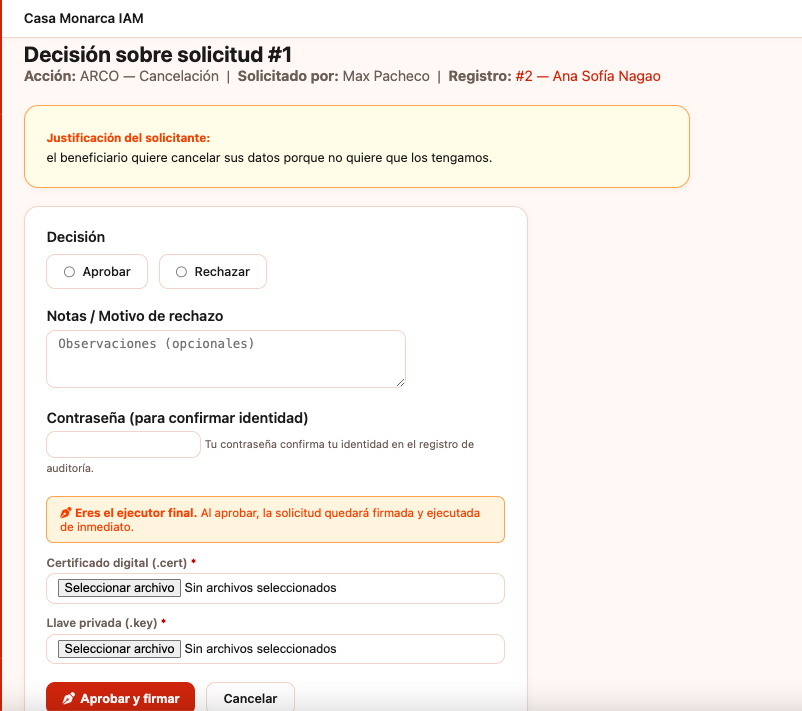
\includegraphics[width=0.85\textwidth]{workflow_decidir.png}
  \caption{Pantalla de decisión de solicitud con firma digital obligatoria (Nivel 1/2).}
  \label{fig:workflow_decidir}
\end{figure}

\section{Ejecutar una solicitud aprobada}

Cuando todas las aprobaciones requeridas se completan, la solicitud queda en estado \textit{Aprobado}. El Administrador hace clic en \textbf{Ejecutar}, ingresa su contraseña y adjunta \texttt{.cert} y \texttt{.key}.

% CAPTURA: pantalla de ejecución con resumen de la solicitud, contraseña y campos de credenciales.
\begin{figure}[H]\centering
  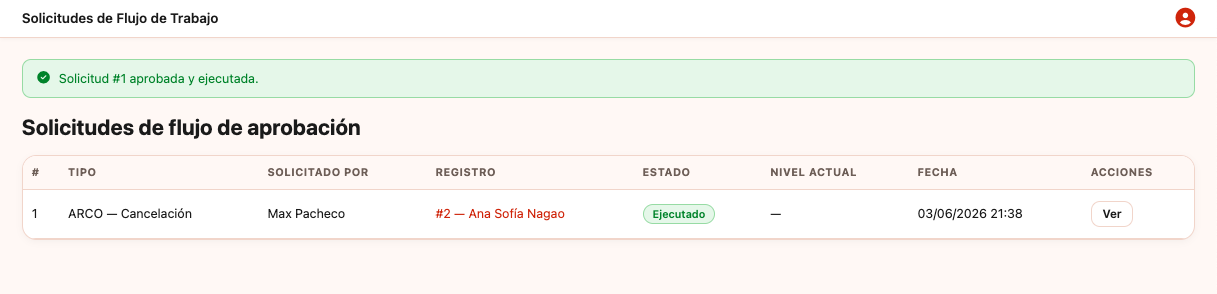
\includegraphics[width=0.85\textwidth]{workflow_ejecutar.png}
  \caption{Pantalla de ejecución de solicitud aprobada con credenciales digitales.}
  \label{fig:workflow_ejecutar}
\end{figure}

% ──────────────────────────────────────────────────────────────────
\chapter{Derechos ARCO}
% ──────────────────────────────────────────────────────────────────
\paraadmin

Los derechos ARCO permiten a los beneficiarios ejercer sus derechos sobre los datos personales registrados en el sistema, conforme a la Ley Federal de Protección de Datos Personales en Posesión de los Particulares (LFPDPPP).

\begin{table}[H]\centering
\caption{Tipos de derechos ARCO y nivel de ejecución requerido.}
\label{tab:arco_tipos}
\begin{tabularx}{\textwidth}{l X l}
\toprule
\textbf{Tipo} & \textbf{Descripción} & \textbf{Ejecuta}\\
\midrule
A · Acceso        & Conocer los datos almacenados sobre el beneficiario. & Coordinador (Nivel 2)\\
R · Rectificación & Corregir datos inexactos; puede adjuntarse PDF de evidencia. & Coordinador (Nivel 2)\\
C · Cancelación   & Eliminar los datos del sistema definitivamente. & \textbf{Solo Admin (Nivel 1)}\\
O · Oposición     & Oponerse a un uso específico de los datos. & Coordinador (Nivel 2)\\
\bottomrule
\end{tabularx}
\end{table}

\section{Listado de solicitudes ARCO}

Menú → \textbf{ARCO}. Muestra todas las solicitudes ARCO registradas en el sistema con su estado actual. Desde aquí también se puede crear una nueva solicitud con el botón \textbf{+ Nueva solicitud ARCO}.

% CAPTURA: pantalla de Solicitudes ARCO con la nota informativa de tipos y quién ejecuta,
%          el listado de solicitudes y el botón "+ Nueva solicitud ARCO".
\begin{figure}[H]\centering
  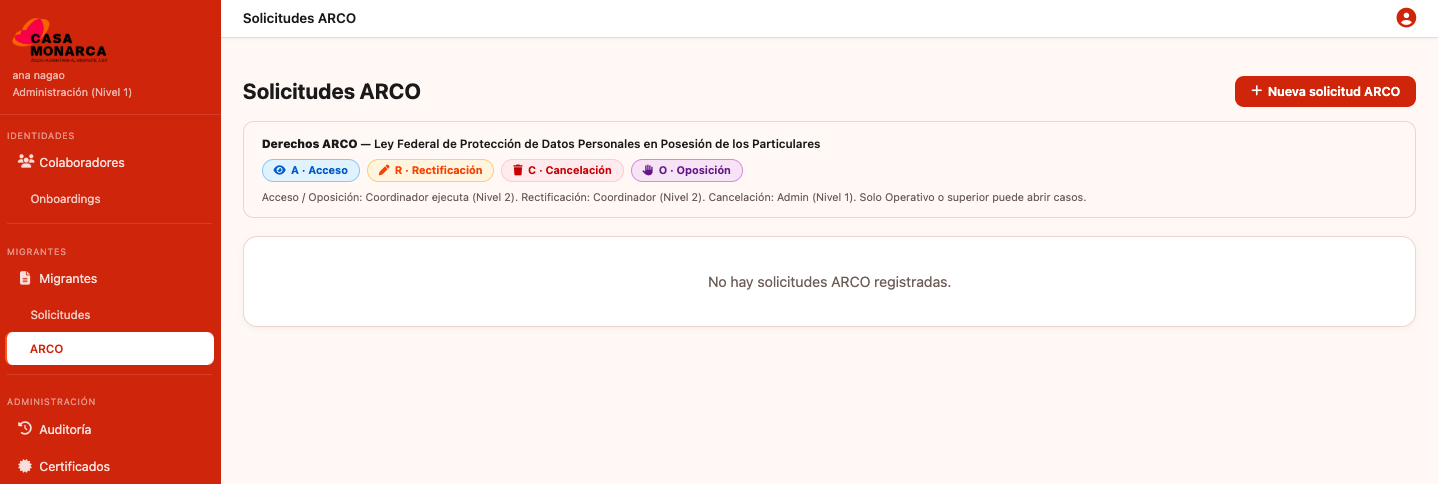
\includegraphics[width=0.95\textwidth]{arco_lista.png}
  \caption{Pantalla de Solicitudes ARCO con los tipos disponibles y el listado de casos.}
  \label{fig:arco_lista}
\end{figure}

\section{Crear una nueva solicitud ARCO}

Una solicitud ARCO se puede iniciar de dos formas:
\begin{itemize}[leftmargin=1.4em]
  \item Desde el \textbf{detalle del registro del migrante} → botón \textbf{Nueva solicitud ARCO}.
  \item Desde el \textbf{listado de ARCO} → botón \textbf{+ Nueva solicitud ARCO}.
\end{itemize}

\paso{1}{Acceder al formulario de nueva solicitud.}

\paso{2}{Seleccionar el tipo de derecho ARCO, escribir una descripción detallada de la solicitud (mínimo 20 caracteres) y, en caso de Rectificación, adjuntar el PDF de evidencia (máx. 5 MB).}

\paso{3}{Enviar la solicitud.}
El sistema registra el caso con un identificador único.

% CAPTURA: formulario de nueva solicitud ARCO (selector de tipo, campo de descripción, adjunto PDF).
\begin{figure}[H]\centering
  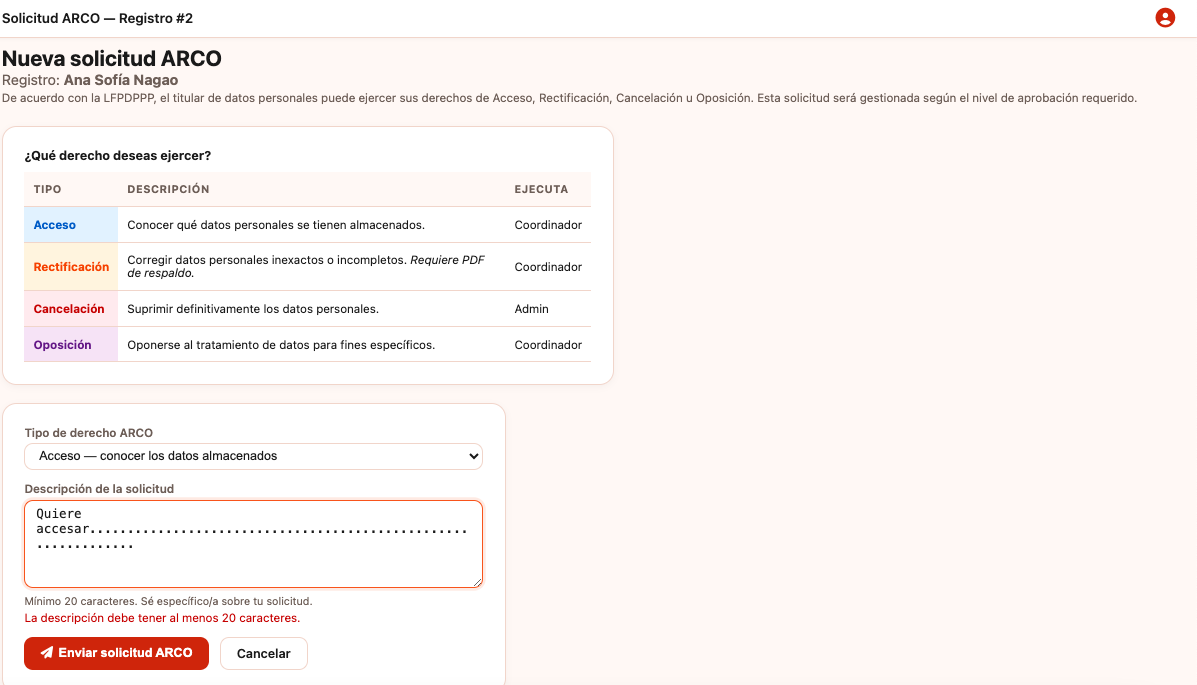
\includegraphics[width=0.85\textwidth]{arco_nueva.png}
  \caption{Formulario de nueva solicitud ARCO con tipo, descripción y documento adjunto.}
  \label{fig:arco_nueva}
\end{figure}

\section{Detalle y ejecución de una solicitud ARCO}

Hacer clic sobre una solicitud del listado para ver su detalle: registro afectado, tipo de derecho, descripción y documento adjunto si existe. Los usuarios autorizados pueden ejecutarla desde esta misma pantalla.

% CAPTURA: vista de detalle de una solicitud ARCO con el registro afectado y las opciones de ejecución.
\begin{figure}[H]\centering
  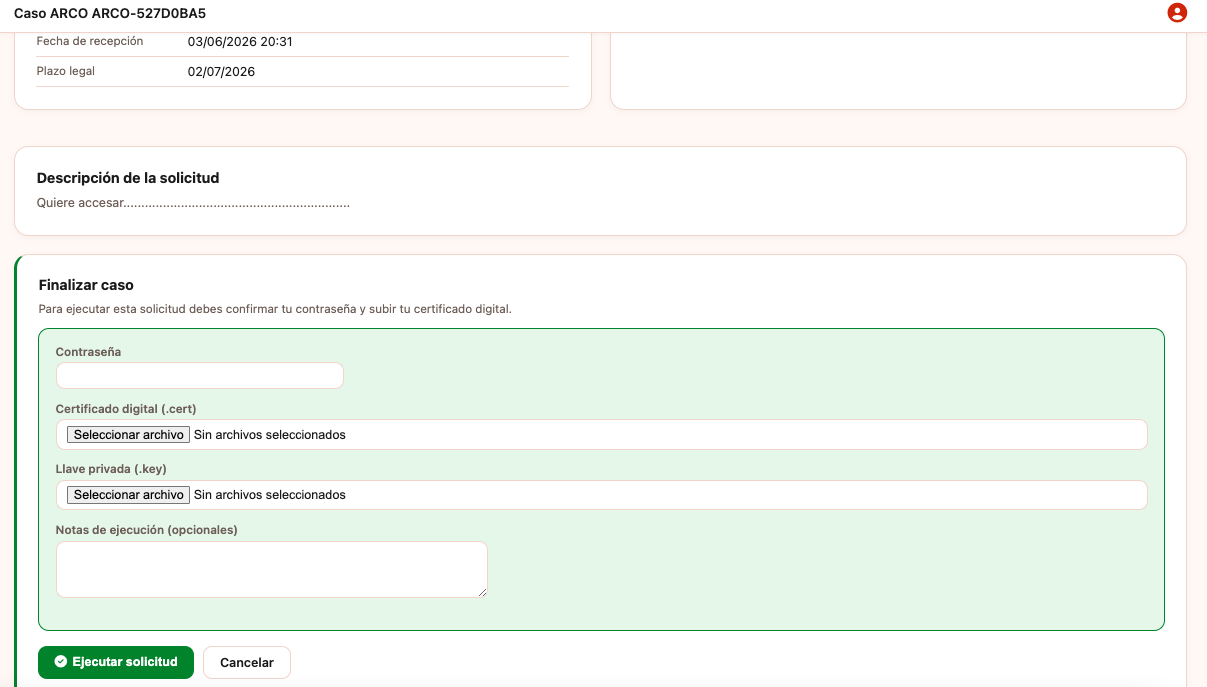
\includegraphics[width=0.95\textwidth]{arco_detalle.png}
  \caption{Vista de detalle de una solicitud ARCO con las opciones de ejecución disponibles.}
  \label{fig:arco_detalle}
\end{figure}

\begin{nota}
La \textbf{Cancelación ARCO} elimina definitivamente los datos del beneficiario del sistema y solo puede ser ejecutada por el Administrador (Nivel 1).
\end{nota}


% ============================================================================
%  PARTE III ─ MANUAL DEL COORDINADOR (Nivel 2)
% ============================================================================
\part{Manual del Coordinador --- Nivel 2}

% ──────────────────────────────────────────────────────────────────
\chapter{Gestión de colaboradores de área}
% ──────────────────────────────────────────────────────────────────
\paracoord

El Coordinador gestiona únicamente los colaboradores de su área y solo puede crear o editar cuentas de Nivel 3 y 4. No puede emitir certificados digitales (eso es exclusivo del Administrador).

\section{Dashboard}

El dashboard muestra los colaboradores del área del Coordinador. Los filtros de área no están disponibles (ya está restringido a la suya). Puede ver los onboardings pendientes de su área.

% CAPTURA: dashboard del Coordinador con los colaboradores de su área y el acceso a onboardings pendientes.
\begin{figure}[H]\centering
  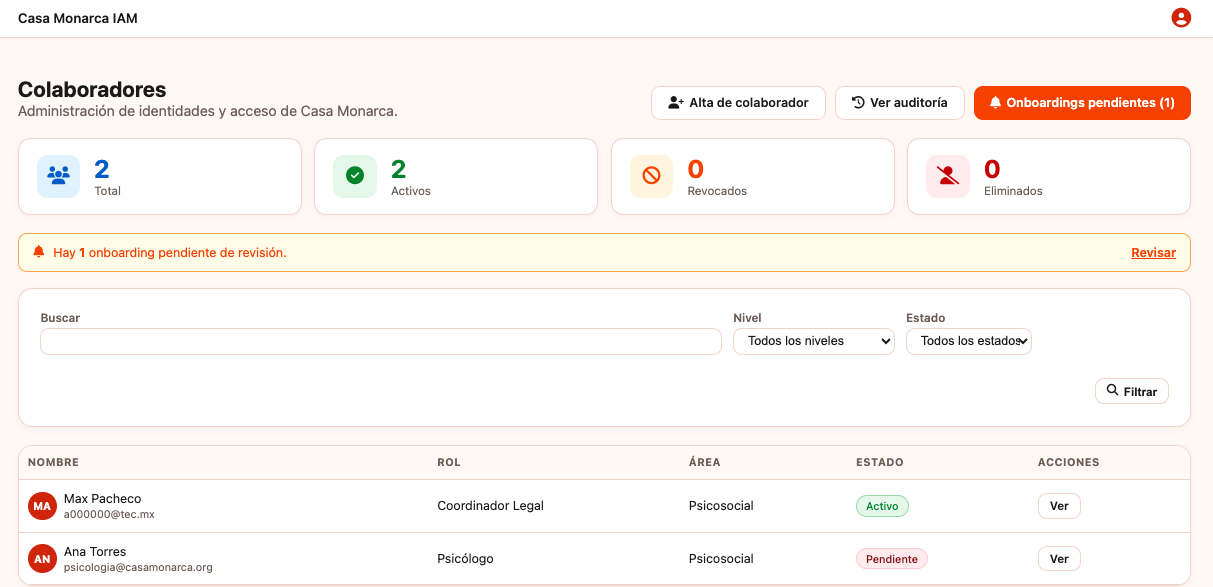
\includegraphics[width=0.95\textwidth]{dashboard_coord.png}
  \caption{Dashboard del Coordinador con los colaboradores de su área.}
  \label{fig:dashboard_coord}
\end{figure}

\section{Dar de alta a un colaborador (Nivel 3 y 4)}

El proceso es idéntico al del Administrador (ver Capítulo~4), con las siguientes restricciones:
\begin{itemize}[leftmargin=1.4em]
  \item Solo puede crear cuentas de Nivel 3 (Operativo) y Nivel 4 (Voluntario).
  \item No puede cambiar el área ni el tipo de cuenta administrador.
  \item La contraseña temporal se genera aleatoriamente y se muestra una sola vez.
\end{itemize}

\section{Gestión de colaboradores del área}

Las acciones disponibles sobre los colaboradores de su área son: Editar datos, Activar/Desactivar, Revocar y Eliminar. Para aprobar onboardings, el proceso requiere contraseña y \texttt{.cert}+\texttt{.key} (ver Sección~\ref{sec:onboarding_comun}).

% ──────────────────────────────────────────────────────────────────
\chapter{Registro de migrantes --- Coordinador}
% ──────────────────────────────────────────────────────────────────
\paracoord

El Coordinador puede crear, editar y eliminar registros de forma directa (igual que el Administrador). Los flujos de formulario, revisión y firma son idénticos a los descritos en el Capítulo~\ref{ch:migrante_admin}. También tiene acceso al expediente completo del migrante (Sección~\ref{sec:expediente}).

% ──────────────────────────────────────────────────────────────────
\chapter{Solicitudes de cambio --- Coordinador}
% ──────────────────────────────────────────────────────────────────
\paracoord

El Coordinador ve las solicitudes generadas en el sistema (no solo las de su área en la versión actual). Puede aprobar, rechazar y ejecutar solicitudes siguiendo el mismo proceso que el Administrador (contraseña + \texttt{.cert} + \texttt{.key} para aprobaciones). La firma masiva también está disponible.

% ──────────────────────────────────────────────────────────────────
\chapter{Derechos ARCO --- Coordinador (revisión y escalación)}
% ──────────────────────────────────────────────────────────────────
\paracoord

El Coordinador puede registrar nuevas solicitudes ARCO, ver el listado de solicitudes y actuar sobre los tickets ARCO que le corresponden.

\section{Revisar una solicitud ARCO}

Menú → \textbf{ARCO} → clic en una solicitud. El detalle muestra la información del caso (ID, tipo de derecho, estado, solicitante, fecha de recepción y plazo legal), el registro afectado (folio interno, nombre y nacionalidad) y la descripción de la solicitud. Al pie aparece el \textbf{Flujo de aprobación} vinculado con su estado actual.

% CAPTURA: detalle de un caso ARCO con las secciones de Información del caso,
%          Registro afectado, Descripción y Flujo de aprobación.
\begin{figure}[H]\centering
  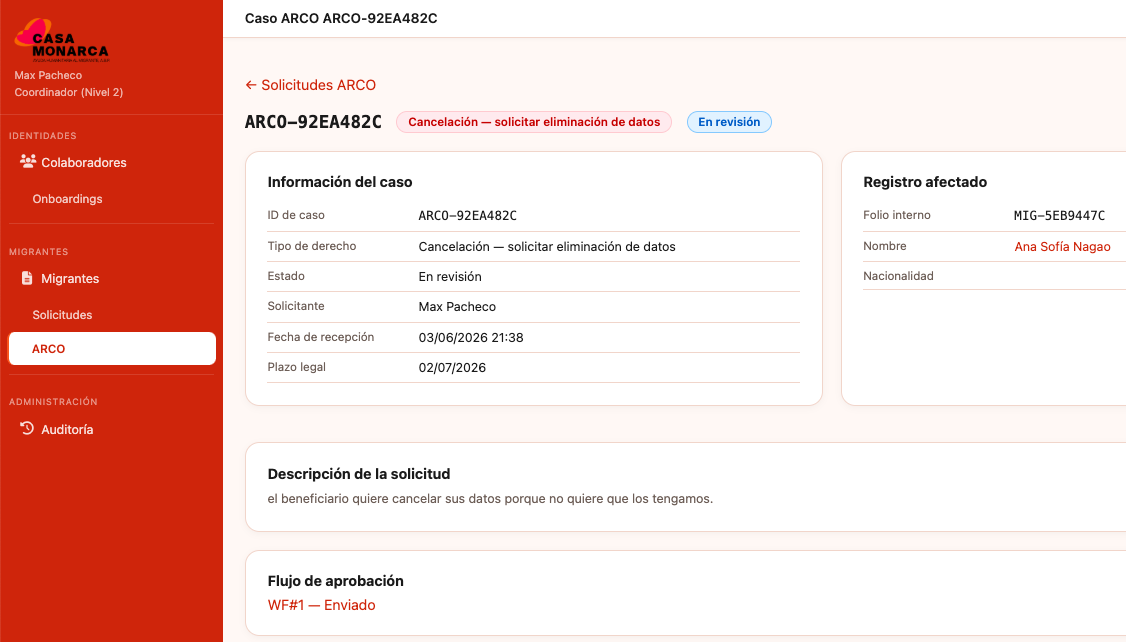
\includegraphics[width=0.95\textwidth]{arco_detalle_coord.png}
  \caption{Vista de detalle de un caso ARCO con la información del caso y el flujo de aprobación vinculado.}
  \label{fig:arco_detalle_coord}
\end{figure}

\begin{nota}
El plazo legal indica la fecha límite para dar respuesta a la solicitud conforme a la normativa de protección de datos personales.
\end{nota}

\section{Rechazar un ticket ARCO}

Si la solicitud no procede, clic en \textbf{Rechazar}, ingresar el motivo de rechazo y confirmar. El ticket pasa a estado \textit{Rechazada}.

\begin{nota}
El Coordinador \textbf{no puede} ejecutar una Cancelación ARCO — esa acción es exclusiva del Administrador (Nivel 1).
\end{nota}

\section{Cadena de auditoría}

El Coordinador también tiene acceso a la cadena de auditoría criptográfica (Menú → \textbf{Cadena de auditoría}).

% ============================================================================
%  PARTE IV ─ MANUAL DEL OPERATIVO (Nivel 3)
% ============================================================================
\part{Manual del Operativo --- Nivel 3}

% ──────────────────────────────────────────────────────────────────
\chapter{Registro de migrantes --- Operativo}
% ──────────────────────────────────────────────────────────────────
\paraoper

El Operativo puede \textbf{registrar nuevos migrantes de forma directa} — no necesita pasar por un workflow para crear. Sin embargo, para editar o eliminar registros existentes debe enviar una solicitud de cambio.

\section{Crear un nuevo registro}

\paso{1}{Menú → \textbf{Nuevo Registro}.}
Se abre el formulario completo idéntico al del Administrador (ver Tabla~\ref{tab:campos_migrante}).

\paso{2}{Completar el formulario y aceptar el Aviso de Privacidad.}

\paso{3}{Enviar.}
El sistema crea una \textbf{solicitud de creación} de registro en el flujo de aprobación y redirige al listado de workflow. El registro quedará activo en el sistema una vez que el Coordinador o Administrador lo apruebe y ejecute.

% CAPTURA: mensaje de confirmación tras envío de solicitud de creación ("Tu solicitud fue enviada. Puedes seguir su estado en el flujo de trabajo.").
\begin{figure}[H]\centering
  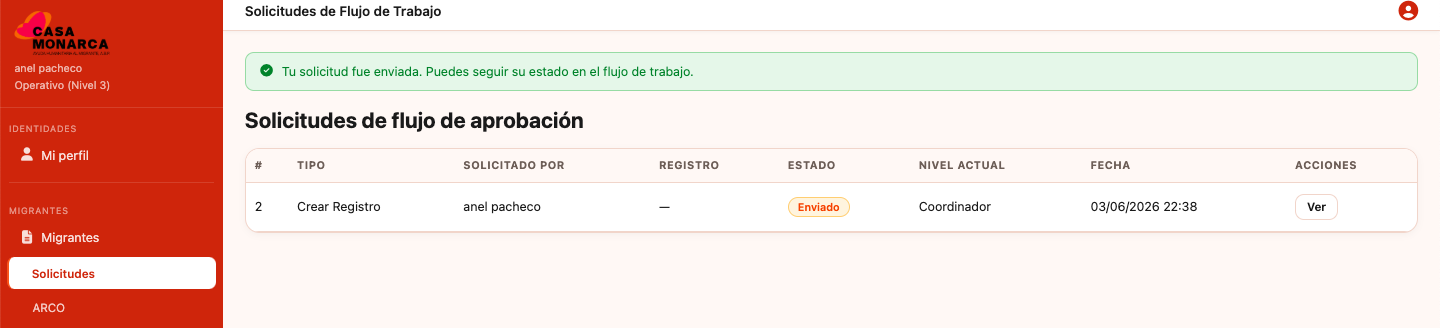
\includegraphics[width=0.75\textwidth]{operativo_solicitud_enviada.png}
  \caption{Confirmación de solicitud de creación enviada al flujo de aprobación (Nivel 3).}
  \label{fig:operativo_solicitud_enviada}
\end{figure}

\section{Ver el listado y el detalle de registros}

El Operativo puede ver el listado de registros activos y el detalle de cualquier expediente (búsqueda por ID interno). Si un registro fue cancelado por ARCO, el acceso devuelve un error.

% ──────────────────────────────────────────────────────────────────
\chapter{Seguimiento de solicitudes y tickets}
% ──────────────────────────────────────────────────────────────────
\paraoper

\section{Solicitudes de cambio (Workflow)}

Menú → \textbf{Solicitudes}. El Operativo ve solo las solicitudes que él mismo generó. Puede ver el detalle de cada una y el historial de pasos de aprobación. Si el flujo de aprobación lo designa como aprobador actual, puede también decidir sobre esa solicitud.

% CAPTURA: listado de solicitudes del Operativo (solo las propias) con estado y fecha.
\begin{figure}[H]\centering
  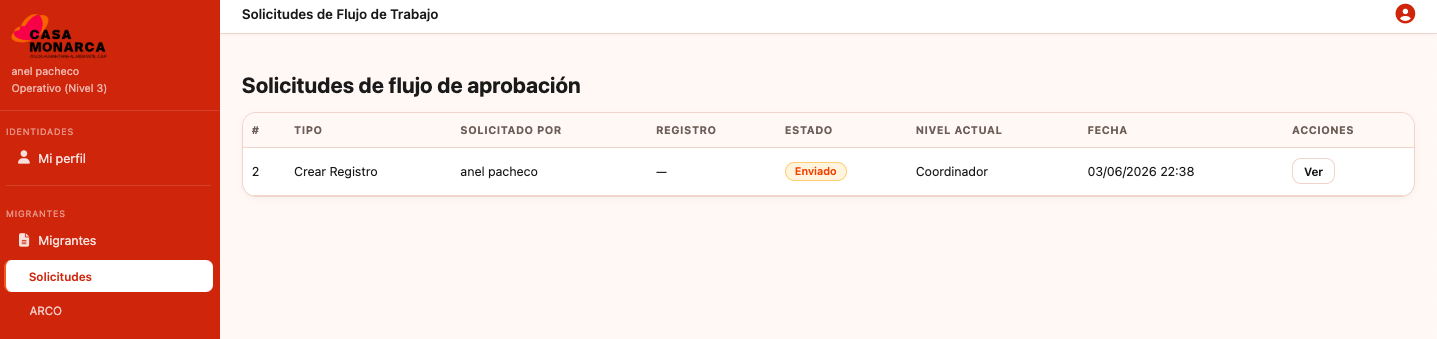
\includegraphics[width=0.95\textwidth]{operativo_workflow_lista.png}
  \caption{Listado de solicitudes de cambio del Operativo (solo las propias).}
  \label{fig:operativo_workflow_lista}
\end{figure}

\section{Tickets de seguimiento}

Menú → \textbf{Tickets}. Muestra los tickets generados por las solicitudes de workflow propias. Solo lectura; el estado lo actualiza el Coordinador o Administrador.

% ──────────────────────────────────────────────────────────────────
\chapter{Derechos ARCO --- Operativo}
% ──────────────────────────────────────────────────────────────────
\paraoper

El Operativo puede crear solicitudes ARCO y ver el estado de las que él mismo registró.

\section{Registrar una solicitud ARCO}

El proceso es idéntico al del Administrador: Menú → \textbf{ARCO} → \textbf{Nueva solicitud ARCO} → seleccionar el migrante por ID interno → completar el formulario → enviar. El sistema crea el ticket ARCO y notifica al Coordinador.

\section{Ver mis solicitudes ARCO}

Menú → \textbf{ARCO}. El listado muestra solo las solicitudes registradas por el propio Operativo con su estado actual.

% ============================================================================
%  PARTE V ─ MANUAL DEL VOLUNTARIO / EXTERNO (Nivel 4)
% ============================================================================
\part{Manual del Voluntario / Externo --- Nivel 4}

% ──────────────────────────────────────────────────────────────────
\chapter{Nueva solicitud de registro de migrante}
% ──────────────────────────────────────────────────────────────────
\paraext

El Voluntario puede llenar el formulario de registro de migrantes. El sistema crea automáticamente una solicitud de creación que el personal de la organización revisará.

\paso{1}{Al iniciar sesión, el sistema redirige directamente al formulario de \textbf{Nuevo Registro}.}

\paso{2}{Completar todos los campos del formulario} (ver Tabla~\ref{tab:campos_migrante}).

\paso{3}{Aceptar el Aviso de Privacidad y hacer clic en \textbf{Enviar}.}

El sistema muestra el mensaje: \textit{``Tu solicitud fue enviada. El operador la revisará pronto.''} y regresa al formulario vacío para una posible nueva solicitud.

% CAPTURA: mensaje de confirmación tras envío ("Tu solicitud fue enviada. El operador la revisará pronto.") y formulario listo para una nueva solicitud.
\begin{figure}[H]\centering
  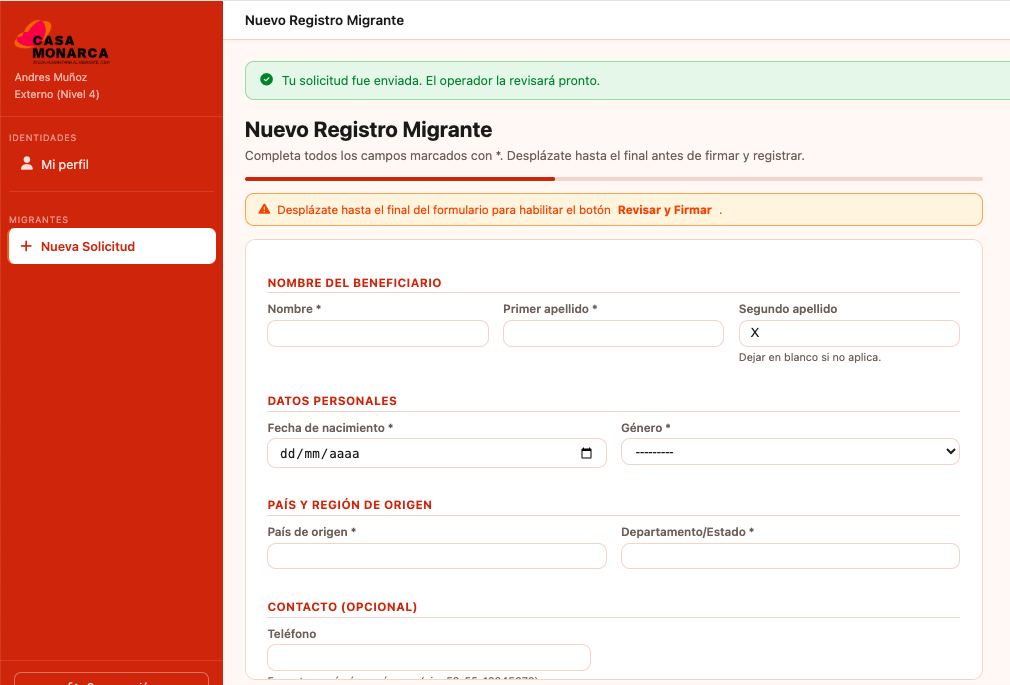
\includegraphics[width=0.75\textwidth]{voluntario_confirmacion.png}
  \caption{Confirmación de solicitud enviada y formulario disponible para nuevo registro (Nivel 4).}
  \label{fig:voluntario_confirmacion}
\end{figure}

\begin{nota}
El Voluntario no tiene acceso al listado de registros ni puede ver el estado de sus solicitudes desde esta interfaz. Para consultar el avance, debe comunicarse con un Operativo o Coordinador.
\end{nota}

\chapter{Roles y permisos}
% ──────────────────────────────────────────────────────────────────

\section{Módulo IAM — Gestión de colaboradores}

\begin{table}[H]\centering
\caption{Permisos en el módulo IAM por nivel.}
\label{tab:permisos_iam}
\begin{tabularx}{\textwidth}{X c c c c}
\toprule
\textbf{Función} & \textbf{Niv. 1} & \textbf{Niv. 2} & \textbf{Niv. 3} & \textbf{Niv. 4}\\
\midrule
Ver todos los colaboradores          & Sí & Solo área & No & No\\
Crear colaboradores Nivel 1–2        & Sí & No & No & No\\
Crear colaboradores Nivel 3–4        & Sí & Sí (área) & No & No\\
Editar / Activar / Revocar / Eliminar & Sí & Sí (área, Niv. 3–4) & No & No\\
Aprobar onboardings                  & Sí & Sí (área) & No & No\\
Gestión de certificados (módulo)     & Sí & No & No & No\\
Emitir certificado (desde detalle)   & Sí & No & No & No\\
Validar certificado                  & Sí & Sí (área) & No & Sí (propio)\\
Ver auditoría IAM                    & Sí (global) & Sí (área) & No & No\\
Requiere \texttt{.cert}+\texttt{.key} para login & Sí & Sí & No & No\\
\bottomrule
\end{tabularx}
\end{table}

\section{Módulo Registros — Migrantes}

\begin{table}[H]\centering
\caption{Permisos en el módulo de migrantes por nivel.}
\label{tab:permisos_migrantes}
\begin{tabularx}{\textwidth}{X c c c c}
\toprule
\textbf{Función} & \textbf{Niv. 1} & \textbf{Niv. 2} & \textbf{Niv. 3} & \textbf{Niv. 4}\\
\midrule
Crear registro (directo)               & Sí & Sí & No & No\\
Crear registro (vía solicitud)         & --- & --- & Sí & Sí\\
Ver listado y detalle                  & Sí & Sí & Sí & No\\
Editar (directo)                       & Sí & Sí & No & No\\
Editar (vía solicitud, 12 campos)      & --- & --- & Sí & Sí\\
Eliminar (directo)                     & Sí & Sí & No & No\\
Eliminar (vía solicitud)               & --- & --- & Sí & Sí\\
Verificar integridad                   & Sí & Sí & Sí & No\\
Expediente completo                    & Sí & Sí & No & No\\
Registros eliminados                   & Sí & No & No & No\\
Aprobar/rechazar workflow              & Sí & Sí & Sí\textsuperscript{*} & No\\
Ejecutar workflow                      & Sí & Sí & No & No\\
Firma masiva                           & Sí & Sí & No & No\\
ARCO: crear/ver                        & Sí & Sí & Sí (propias) & Sí (propias)\\
ARCO: ejecutar (Acceso/Rectif./Oposición) & Sí & Sí & No & No\\
ARCO: ejecutar (Cancelación)           & Sí & No & No & No\\
ARCO tickets: revisar+escalar          & --- & Sí & No & No\\
ARCO tickets: aprobar+ejecutar         & Sí & No & No & No\\
ARCO tickets: rechazar                 & Sí & Sí & No & No\\
ARCO cancelados                        & Sí & Sí & No & No\\
Cadena de auditoría                    & Sí & Sí & No & No\\
Tickets (ver)                          & Sí (todos) & Sí (todos) & Sí (propios) & No\\
\bottomrule
\end{tabularx}
\end{table}
{\small \textsuperscript{*} El Operativo puede decidir sobre solicitudes solo si el flujo lo designa como aprobador actual en la cadena.}

% ──────────────────────────────────────────────────────────────────
\chapter{Solución de problemas}
% ──────────────────────────────────────────────────────────────────

\begin{longtable}{p{0.52\textwidth} p{0.43\textwidth}}
\caption{Mensajes de error comunes y acciones recomendadas.}\label{tab:errores}\\
\toprule
\textbf{Mensaje de error} & \textbf{Acción recomendada}\\
\midrule
\endfirsthead
\toprule
\textbf{Mensaje de error} & \textbf{Acción recomendada}\\
\midrule
\endhead
\bottomrule
\endfoot
Usuario no encontrado.                         & Verificar el nombre de usuario.\\
Contraseña incorrecta.                         & Revisar mayúsculas y caracteres especiales.\\
Demasiados intentos fallidos...                & Esperar 15 minutos o contactar al administrador.\\
Tu cuenta ha sido revocada. Contacta al administrador. & Comunicarse con el área de TI.\\
Tu cuenta está inactiva. Contacta al administrador. & Solicitar reactivación al administrador.\\
Esta cuenta ha sido eliminada. Contacta al administrador. & Crear cuenta nueva si aplica.\\
Los administradores y coordinadores deben proporcionar el certificado digital (.cert) y la llave privada (.key). & Seleccionar ambos archivos en el login.\\
El certificado digital o la llave privada son inválidos. & Verificar que sean los archivos originales sin modificar.\\
Certificado o llave inválidos. Usa el .cert y la .key originales descargados... & Usar exactamente los archivos descargados; no convertirlos.\\
El certificado aún no está disponible.         & Esperar a que el administrador emita el certificado.\\
Respuesta incorrecta. Inténtalo de nuevo.      & Reintentar la respuesta de seguridad.\\
La validación del certificado falló.           & Certificado revocado o expirado; contactar al administrador.\\
Contraseña incorrecta. No se pudo firmar la aprobación. & Verificar la contraseña al firmar.\\
Debes subir tu certificado digital y tu llave privada para ejecutar. & Adjuntar ambos archivos en la pantalla de ejecución.\\
Formato inválido. Usa: +país-área-número (ej: +52-55-12345678). & Corregir el formato del teléfono.\\
Solo se aceptan archivos PDF.                  & Convertir el documento a PDF antes de cargarlo.\\
El archivo no puede superar los 5 MB.         & Comprimir o reducir el archivo PDF.\\
La descripción debe tener al menos 20 caracteres. & Ampliar la descripción de la solicitud ARCO.\\
No tienes permisos para acceder a esta sección. & Verificar el nivel de acceso asignado.\\
El ticket no está en estado para revisar.      & Recargar la página y verificar el estado actual del ticket.\\
Solo el Administrador puede ejecutar una Cancelación ARCO. & Escalar al Administrador.\\
\end{longtable}

% ──────────────────────────────────────────────────────────────────
\chapter{Preguntas frecuentes}
% ──────────────────────────────────────────────────────────────────

\subsection*{¿Qué hago si olvidé mi contraseña?}
Usar la opción de recuperación en la pantalla de login. Se pide el usuario y la respuesta a la pregunta de seguridad. Si no hay pregunta configurada, contactar al administrador.

\subsection*{¿Dónde veo la contraseña temporal de un colaborador recién creado?}
Se muestra una única vez en la pantalla de confirmación posterior al alta. No vuelve a mostrarse; copiarla y entregarla de forma segura en ese momento.

\subsection*{¿Por qué no puedo iniciar sesión si mi cuenta existe?}
Las causas más comunes son: cuenta inactiva, revocada o eliminada; bloqueo temporal por intentos fallidos; o falta del \texttt{.cert}/\texttt{.key} en cuentas de Nivel 1 y 2. El mensaje en pantalla indica el motivo exacto.

\subsection*{¿Dónde guardo los archivos .cert y .key?}
En un lugar seguro y de acceso restringido. Son necesarios en cada inicio de sesión de Nivel 1 y 2. No modificarlos ni convertirlos a otro formato.

\subsection*{¿Por qué no puedo buscar registros de migrantes por nombre?}
Los campos de nombre y apellidos están \textbf{cifrados} en la base de datos por privacidad. La búsqueda solo es posible por el \textbf{identificador interno} del expediente (\texttt{CM-XXXXXXXX}).

\subsection*{¿Qué diferencia hay entre suspender y revocar un certificado?}
Suspender es temporal y reversible (se puede reactivar con la misma llave). Revocar es permanente e irreversible; el certificado queda inválido para siempre.

\subsection*{¿Qué diferencia hay entre los tickets regulares y los tickets ARCO?}
Los tickets regulares hacen seguimiento de las solicitudes de workflow (creación, edición, eliminación de registros). Los tickets ARCO son específicos para las solicitudes de derechos de privacidad y tienen su propio flujo de dos niveles (Coordinador revisa → Administrador ejecuta).

\subsection*{¿Por qué mi edición de registro no se aplicó de inmediato?}
Los usuarios de Nivel 3 y 4 no pueden editar directamente; el sistema genera una solicitud de actualización que debe ser aprobada y ejecutada por un Coordinador o Administrador.

\subsection*{¿Puedo cambiar mi pregunta de seguridad o mi contraseña?}
Sí. La pregunta de seguridad: menú de perfil → \textbf{Cambiar pregunta de seguridad}. La contraseña: menú de perfil → \textbf{Cambiar contraseña}. Ambas están disponibles en cualquier momento con la sesión activa.

\subsection*{¿Qué pasa con un registro cancelado por ARCO (Cancelación)?}
El expediente se marca como cancelado y desaparece del listado activo. Solo el Administrador puede verlo en el historial de cancelados para cumplimiento de auditoría. Los datos cifrados del beneficiario quedan suprimidos del sistema operativo.

\end{document}